\addtocontents{toc}{\protect\newpage}
\chapter[Flux-limited Diffusion for Multiple Scattering in Participating Media]{Flux-limited Diffusion for Multiple Scattering in Participating Media\\[15pt]\normalsize\itshape This chapter is based on the publication Flux-limited Diffusion for Multiple Scattering in\\[-13pt] Participating Media~\cite{Koerner14}}
\chaptermark{Flux-limited Diffusion}
\label{sec:fld}

In the previous chapter, the angular variable of the radiative transfer equation was discretized into a set of coupled partial differential equations, namely the $P_N$-equations. Furthermore, the chapter introduced a discretization of these equations into a system of linear equations, which could be solved using standard methods. Since the number of equations depends on the truncation order $N$, higher $N$ will result in increasingly larger systems. The results showed that the amount of computational resources required makes this approach unattractive for practical rendering applications, especially for higher $N$ (section~\ref{sec:pn_results}).

In this chapter, flux-limited diffusion is introduced to solve the problem of rendering participating media in computer graphics. The theory has been invented in the astrophysics domain and is primarily attributed to Levermore et al.~\cite{Levermore81}. Their work introduces the theory and discusses its properties for certain canonical problems, such as a single point source within a homogeneous participating medium. In this chapter, a novel numerical method is devised, based on flux-limited diffusion theory. It allows solving for the fluence on a finite difference grid with higher accuracy at a significantly lower cost than $P_1$.

In order to derive the theory for flux-limited diffusion, we will switch in this chapter to a different way of expressing the spherical harmonics expansion. This alternative representation is called \emph{moment expansion}. It is more efficient in regards to notation for lower order $N$ and allows to present the theory more intuitively.

In section \ref{sec:da_moment_expansion_L} and \ref{sec:da_moment_expansion_RTE}, we introduce the moment expansion for the radiance field and radiative transfer equation respectively. The section \ref{sec:moment_closure} follows by introducing the \emph{moment closure problem} and its naive solution, which gives rise to the diffusion approximation. The diffusion approximation is discussed in section~\ref{sec:diffusion_approximation}. It is a method for solving the $P_N$-equations for order $N=1$ very efficiently and it is an important building block for the theory of flux-limited diffusion.

The chapter then continues by revisiting the moment closure problem from section~\ref{sec:moment_closure} and introduces the flux-limit constraint, which is violated by diffusion and causes energy loss. The streaming transport regime is introduced, for which an advection style equation is derived in section~\ref{sec:fld_streaming_limit_approximation}. Flux-limited diffusion is derived as a means to blend between the two extreme modes of transport using local information. This blending is driven by the variable Eddington factor, which is introduced in section~\ref{sec:fld_vef}. Various concrete realizations of the Eddington factor are given and compared in section~\ref{sec:fld_vef_factors}. Finally, an iterative solver is presented in section~\ref{sec:fld_solver}, for which results are presented in section~\ref{sec:fld_results}. The chapter closes with a discussion in section~\ref{sec:fld_discussion}.



\section{Moment Expansion of the Radiance Field}
\label{sec:da_moment_expansion_L}

In section~\ref{sec:sh} it has been established that spherical functions can be represented using a linear combination of spherical harmonics basis functions (equation~\ref{eq:sh_reconstruction}). The coefficients of these basis functions are found by projection (equation~\ref{eq:sh_projection}). Another option for representing spherical functions is the coordinate free form given by tensor calculus. This form is derived by representing the spherical harmonics basis functions themself as linear combination of products of the components of the basis vectors, which establish the underlying coordinate system. Because this representation allows to change the coordinate system independently from the representation, it is referred to as being coordinate free. For a refresher on tensor calculus, an introductory standard such as Grinfeld~\cite{Grinfeld13} is recommended. As with the spherical harmonics expansion, the coordinate free representation can be found for the radiance field as well as the individual terms of the radiative transfer equation. This is referred to as the moment expansion or multipole expansion of the radiance field and the radiative transfer equation respectively.

The moment expansion is a different approach to represent the spherical harmonics expansion of the radiance field and the radiative transfer equation. Its benefit lies in its notational efficieny, especially for lower order. However, for truncation order of $N=2$ and higher, it introduces additional redundancy which makes the standard spherical harmonics expansion much better suited when deriving computational methods from the theory, such as the $P_N$-method in chapter~\ref{sec:pnmethod}. Because the flux-limited diffusion is related to the first order truncation $N=1$, the moment expansion is the standard way of representing the theory. No additional redundancy is introduced and the notational efficiency allows to express the underlying intuition easier.

The moment expansion is derived starting from the spherical harmonics reconstruction of the radiance field:
\begin{align}
\label{eq:fld_moment_expansion_sh_expansion}
L\left(\vec{\omega}\right) =
\sum_{l=0}^{\infty}\sum_{m=-l}^{l}L^{l,m}\SHBC^{l,m}
\left(\vec{\omega}\right)
\end{align}
with $L^{l,m}$ being the spherical harmonics basis function coefficients, which are found by spherical harmonics projection (equation~\ref{eq:sh_projection}).

The main step in the derivation of the moment expansion is the replacement of the spherical harmonics basis function $\SHBC^{l,m}$ by a sum of tensor contractions:
\begin{align}
\label{eq:fld_moment_expansion_sum}
\SHBC^{l,m}(\vec{\omega}) =
\sum_{j=0}^\infty{y^{l,m}_j\odot N_j(\vec{\omega})}
\end{align}
The operator symbol $\odot$ denotes a tensor contraction. In this instance, it is a sum over products of the individual components of the tensors $y^{l,m}_j$ and $N_j$. Therefore, each contraction collapses into a scalar value. These values are then added up over all moments $j$. The tensor $N_j$ is a tensor of rank $j$ with $N_0=1$, and is constructed by a sequence of outer products of the direction vector $\vec{\omega}$:
\begin{align}
N_j\left(\vec{\omega}\right)
=N_{k_1, k_2, ..., k_{j-1}, k_j} 
=\vec{\omega}_{k_1}\vec{\omega}_{k_2}...\vec{\omega}_{k_{j-1}}\vec{\omega}_{k_j} 
\end{align}
The index set $\{k_1, k_2, ..., k_{j-1}, k_j\}$ identifies specific tensor components, with each index running over all components of $\vec{\omega}$ ($k_i \in \{x, y, z\}$).

The tensors $y^{l,m}_j$ are found by expanding $\SHBC^{l,m}(\vec{\omega})$ into a sum of tensor components of $N_j$. The factors to these components can be easily extracted and constitute the components of $y^{l,m}_j$. An expansion is possible by using the following non-recursive definition of the Legendre-polynomial, which is derived with the use of the multiple-angle formula\footnote{\url{http://mathworld.wolfram.com/Multiple-AngleFormulas.html} (date of access: 07/26/2018)}:
\begin{align}
P^{lm}(\theta, \phi) = \operatorname{sin}^m(\phi)\sum_j^{\lfloor\frac{l-m}{2}\rfloor}a^{lmj}\operatorname{cos}^{l-m-2j}(\theta)
\qquad \text{for } m \ge 0
\end{align}
Inserting this into the definition of the spherical harmonics basis function $\SHBC^{l,m}$ (equation~\ref{eq:sh_definition_C}) results in:
\begin{align}
\SHBC^{l,m}(\theta, \phi) = C^{l,m}\left(e^{i\phi}\operatorname{sin}\left(\phi\right)\right)^m \sum_j^{\lfloor\frac{l-m}{2}\rfloor}a^{lmj}\operatorname{cos}^{l-m-2j}(\theta)
\qquad \text{for } m \ge 0
\end{align}
As a next step $\SHBC^{l,m}$ will be expressed in terms of unit direction vector $\vec{\omega}$, instead of spherical coordinates. This is done by using the identity $e^{i\phi}\operatorname{sin}\left(\phi\right) = \vec{\omega}_x + i\vec{\omega}_y$ and $\operatorname{cos}(\theta) = \vec{\omega}_z$:
\begin{align}
\SHBC^{l,m}(\vec{\omega}) &=  C^{l,m}\left( \vec{\omega}_x + i\vec{\omega}_y\right)^m \sum_j^{\lfloor\frac{l-m}{2}\rfloor}a^{lmj}\vec{\omega}_z^{l-m-2j}
&\qquad \text{for } m \ge 0
\label{eq:da_moment_expansion_L_shbasis2}
\\
&= \left(-1\right)^m\overline{\SHBC^{l,\abs{m}}}
&\qquad \text{for } m < 0
\end{align}
Expanding the expression for concrete values of $l$ and $m$, will give a sequence of terms, which involve components of $N_j$, multiplied with specified factors. By seeing the expanded formula as a tensor contraction, the components of $y^{l,m}_j$ can be extracted. For $l=0$ and $m=0$ equation~\ref{eq:da_moment_expansion_L_shbasis2} results in:
\begin{align}
\SHBC^{0,0}(\vec{\omega}) = C^{{0,0}}a^{{0,0,0}} = \frac{1}{\sqrt{4\pi}}N_0\quad,
\end{align}
from wich the following can be inferred:
\begin{align}
y^{0,0}_0 = \frac{1}{\sqrt{4\pi}}
\end{align}
For $l=1$ the result is:
\begin{align}
\SHBC^{1,0}(\vec{\omega}) &= C^{{1,0}}a^{{1,0,0}}\vec{\omega}_z = \sqrt{\frac{3}{4\pi}}\vec{\omega}_z
\\
\SHBC^{1,1}(\vec{\omega}) &= C^{{1,1}}a^{{1,1,0}}\vec{\omega}_x+C^{{1,1}}a^{{1,1,0}}\vec{\omega}_yi = -\sqrt{\frac{3}{8\pi}}\vec{\omega}_x - \sqrt{\frac{3}{8\pi}}\vec{\omega}_yi
\\
\SHBC^{1,-1}(\vec{\omega}) &= -\overline{\SHBC^{1,1}}(\vec{\omega})
= \sqrt{\frac{3}{8\pi}}\vec{\omega}_x - \sqrt{\frac{3}{8\pi}}\vec{\omega}_yi
\end{align}
From which the following can be inferred:
\begin{align}
y^{1,-1}_1 = \begin{pmatrix}\sqrt{\frac{3}{8\pi}}  \\ -\sqrt{\frac{3}{8\pi}}i \\ 0 \end{pmatrix}
\qquad
y^{1,0}_1 = \begin{pmatrix}0  \\ 0 \\ \sqrt{\frac{3}{4\pi}} \end{pmatrix}
\qquad
y^{1,1}_1 = \begin{pmatrix}-\sqrt{\frac{3}{8\pi}}  \\ -\sqrt{\frac{3}{8\pi}}i \\ 0 \end{pmatrix}
\end{align}
This scheme continues and becomes more involved for higher moments. For example with $l=3$ an $m=0$:
\begin{align}
\SHBC^{3,0}(\vec{\omega}) &= \underbrace{C^{{3,0}}a^{{3,0,0}}}_{\in y^{3,0}_3}{\vec{\omega}_z}^{3}+\underbrace{C^{{3,0}}a^{{3,0,1}}}_{\in y^{3,0}_1}\vec{\omega}_z
\end{align}
Here a term containing ${\vec{\omega}_z}^{3}$ is presented, which is an element of $N_3$ and another term containing $\vec{\omega}_z$, which is an element of $N_1$. This shows the expression of the the spherical harmonics basis functions as a sum over tensor contractions of different ranks, as Equation~\ref{eq:fld_moment_expansion_sum}.

Inserting equation~\ref{eq:fld_moment_expansion_sum} into equation~\ref{eq:fld_moment_expansion_sh_expansion} gives:
\begin{align}
L\left(\vec{\omega}\right) =
\sum_{l=0}^{\infty}\sum_{m=-l}^{l}L^{l,m}\sum_{j=0}^\infty{y^{l,m}_j\odot N_j(\vec{\omega})}
\end{align}
After rearranging terms that leads to:
\begin{align}
L\left(\vec{\omega}\right) =
\sum_{l=0}^{\infty}\sum_{m=-l}^{l}\sum_{j=0}^\infty{L^{l,m}y^{l,m}_j\odot N_j(\vec{\omega})}
\end{align}
For each spherical harmonics basis $l,m$, all rank $j$ tensors will be iterated, and contracted with their respective $N_j$ (after applying the respective spherical harmonics coefficient as weight). Since the indices $l$ and $j$ run over the same range, this can be swapped. This is identical to rearranging the order of terms:
\begin{align}
L\left(\vec{\omega}\right) =
\sum_{l=0}^{\infty}\underbrace{\sum_{j=0}^\infty\sum_{m=-j}^{j}{L^{j,m}y^{j,m}_l}}_{=f_l}
\odot N_l(\vec{\omega})
\end{align}
For each spherical harmonics band $l$, all spherical harmonics bases $j,m$ will be iterated, weighted and the rank $l$ tensor of each particular basis contracted with $N_l$. Further, the sum of equal rank tensors can be factorized into the moment tensor $f_l$ to receive the moment expansion of the radiance field:
\begin{align}
L\left(\vec{\omega}\right) =
\sum_{l=0}^{\infty}f_l\odot N_l(\vec{\omega})
\end{align}
with
\begin{align}
f_l = \sum_{j=0}^\infty\sum_{m=-j}^{j}{L^{j,m}y^{j,m}_l}
\end{align}
For $f_0$ we get:
\begin{align}
f_0 &= L^{0,0}y^{0,0}_0 = \int_\Omega{L\left(\vec{\omega}\right)\SHBC^{0,0}\left(\vec{\omega}\right)\ud\vec{\omega}}\frac{1}{\sqrt{4\pi}}\\
&=
\frac{1}{4\pi}\int_\Omega{L\left(\vec{\omega}\right)\ud\vec{\omega}} =
\frac{1}{4\pi}\phi
\end{align}
For $f_1$, $L^{1,-1}y^{1,-1}_1$, $L^{1,0}y^{1,0}_1$ and $L^{1,1}y^{1,1}_1$ shall be added. Starting with $L^{1,-1}y^{1,-1}_1$, following result is given:
\begin{align}
L^{1,-1}y^{1,-1}_1 &= 
\int_\Omega{L\left(\vec{\omega}\right)\SHBC^{1,-1}\left(\vec{\omega}\right)\ud\vec{\omega}}
\begin{pmatrix}\sqrt{\frac{3}{8\pi}}  \\ -\sqrt{\frac{3}{8\pi}}i \\ 0 \end{pmatrix}
\\
&= 
\frac{3}{8\pi}\int_\Omega{L\left(\vec{\omega}\right)\operatorname{sin}\theta e^{-i\phi}\ud\vec{\omega}}
\begin{pmatrix}1  \\ -i \\ 0 \end{pmatrix}
\end{align}
Using the trigonometric identities $e^{-i\phi} = \operatorname{cos}\phi - i\operatorname{sin}\phi$ and $e^{i\phi} = \operatorname{cos}\phi + i\operatorname{sin}\phi$, the outcome is:
\begin{align}
L^{1,-1}y^{1,-1}_1 &= 
\begin{pmatrix}
\frac{3}{8\pi}\int_\Omega{L\left(\vec{\omega}\right)\operatorname{sin}\theta\operatorname{cos}\phi\ud\vec{\omega}} - \frac{3}{8\pi}i\int_\Omega{L\left(\vec{\omega}\right)\operatorname{sin}\theta\operatorname{sin}\phi\ud\vec{\omega}}
\\
-\frac{3}{8\pi}i\int_\Omega{L\left(\vec{\omega}\right)\operatorname{sin}\theta\operatorname{cos}\phi\ud\vec{\omega}} - \frac{3}{8\pi}\int_\Omega{L\left(\vec{\omega}\right)\operatorname{sin}\theta\operatorname{sin}\phi\ud\vec{\omega}}
\\
0
\end{pmatrix}
\end{align}
We then use the identity:
\begin{align}
\vec{\omega} &= 
\begin{pmatrix}
\operatorname{sin}\theta\operatorname{cos}\phi
\\
\operatorname{sin}\theta\operatorname{sin}\phi
\\
\operatorname{cos}\theta
\end{pmatrix}\ ,
\end{align}
to arrive at:
\begin{align}
L^{1,-1}y^{1,-1}_1 &= 
\begin{pmatrix}
\frac{3}{8\pi}\int_\Omega{L\left(\vec{\omega}\right)\vec{\omega}_x\ud\vec{\omega}} - \frac{3}{8\pi}i\int_\Omega{L\left(\vec{\omega}\right)\vec{\omega}_y\ud\vec{\omega}}
\\
-\frac{3}{8\pi}i\int_\Omega{L\left(\vec{\omega}\right)\vec{\omega}_x\ud\vec{\omega}} - \frac{3}{8\pi}\int_\Omega{L\left(\vec{\omega}\right)\vec{\omega}_y\ud\vec{\omega}}
\\
0
\end{pmatrix}
\end{align}
Similar procedures for $L^{1,0}y^{1,0}_1$ and $L^{1,1}y^{1,1}_1$, lead to:
\begin{align}
L^{1,0}y^{1,0}_1 &= 
\begin{pmatrix}
0\\
0\\
\frac{3}{4\pi}\int_\Omega{L\left(\vec{\omega}\right)\vec{\omega}_z\ud\vec{\omega}}
\end{pmatrix}
\end{align}
and
\begin{align}
L^{1,1}y^{1,1}_1 &= 
\begin{pmatrix}
\frac{3}{8\pi}\int_\Omega{L\left(\vec{\omega}\right)\vec{\omega}_xi\ud\vec{\omega}} + \frac{3}{8\pi}i\int_\Omega{L\left(\vec{\omega}\right)\vec{\omega}_y\ud\vec{\omega}}
\\
\frac{3}{8\pi}i\int_\Omega{L\left(\vec{\omega}\right)\vec{\omega}_xi\ud\vec{\omega}} + \frac{3}{8\pi}\int_\Omega{L\left(\vec{\omega}\right)\vec{\omega}_y\ud\vec{\omega}}
\\
0
\end{pmatrix}
\end{align}
Subsequently $f_1$ can be merged. Note how all the imaginary terms cancel out:
\begin{align}
f_1 &= 
L^{1,-1}y^{1,-1}_1+L^{1,0}y^{1,0}_1+L^{1,1}y^{1,1}_1
=
\frac{3}{4\pi}
\begin{pmatrix}
\int_\Omega{L\left(\vec{\omega}\right)\vec{\omega}_x\ud\vec{\omega}}
\\
\int_\Omega{L\left(\vec{\omega}\right)\vec{\omega}_y\ud\vec{\omega}}
\\
\int_\Omega{L\left(\vec{\omega}\right)\vec{\omega}_z\ud\vec{\omega}}
\end{pmatrix}
=
\frac{3}{4\pi}\vec{E}
\end{align}
With $f_0$ and $f_1$, the moment expansion of the radiance field truncated after the first moment can be written down and used for reconstruction in the diffusion approximation:
\begin{align}
\nonumber
L\left(\vec{\omega}\right) &= 
f_0\odot N_0 + f_1\odot N_1
\\
\nonumber
&=
\frac{1}{4\pi}\phi + \frac{3}{4\pi}\vec{E} \odot \vec{\omega}
\\
\label{eq:moment_expansion_L}
&=
\frac{1}{4\pi}\phi + \frac{3}{4\pi}\left(w \cdot \vec{E}\right)
\end{align}
The tensor $f_0$ is expressed in terms of the fluence $\phi$ and the tensor $f_1$ in terms of the flux vector $\vec{E}$. These quantities are often referred to as the zero and first moment of the radiance field respectively, generalize to higher order and are denoted $L_i$. They are computed using the moment projection operator $\mu_i$:
\begin{align}
\label{eq:moment_expansion_mu}
\mu_i\left[L\right] = L_i = \int_\Omega{L\left(\vec{\omega}\right)N_i\left(\vec{\omega}\right)\ud\vec{\omega}}
\end{align}
An important quantity for deriving flux-limited diffusion is the second moment of the radiance field, the radiative pressure tensor $L_2$. Its intuition is very similar to the stress tensor in continuum mechanics.


\section{Moment Expansion of the Radiative Transfer Equation}
\label{sec:da_moment_expansion_RTE}

As with the radiance field, the radiative transfer equation can be developed into its moments. The result is a concise representation of the $P_N$-equations, which are particularily expressive for lower truncation order, such as $P_1$. The derivation steps of the spherical harmonics expansion replaced the radiance field quantity in the RTE by its truncated expansion, followed by the expansion of the individual terms of the RTE. The derivation steps of the moment expansion are similar with the difference that the moment expansion (equation~\ref{eq:moment_expansion_mu}) is applied to the RTE terms (equation~\ref{eq:rte}) first and the replacement is done as a second step.

The $n$-th moment of the RTE is found by applying the moment projection operator $\mu_n$ to all the terms of the RTE:
\begin{align*}
\mu_n\left[(\vec{\omega}\cdot\nabla)L(\vec{x}, \vec{\omega})\right]=&\\
\mu_n\left[-\sigma_t(\vec{x})L(\vec{x}, \vec{\omega}) + \sigma_s(\vec{x})\int_{\Omega}\phase(\vec{x}, \vec{\omega}'\rightarrow\vec{\omega})L(\vec{x}, \vec{\omega}')\ud\vec{\omega}' + Q(\vec{x}, \vec{\omega})\right]
%\label{eq:rte_ani}
\end{align*}
Since $\mu_n$ is linear, the LHS gives:
\begin{align*}
\mu_n[(\vec{\omega} \cdot \nabla)L(\vec{x}, \vec{\omega})] & = \int_{\Omega}{(\vec{\omega}\cdot\nabla)L(\vec{x}, \vec{\omega})N_n\ud\vec{\omega}}\\
							     & =\nabla\int_{S^2}{L(\vec{x}, \vec{\omega})N_n\vec{\omega}\ud\vec{\omega}} \\
							     & =\nabla\mu_{n+1}\left[L\right]
\end{align*}
The term $\nabla\mu_{n+1}$ is a tensor divergence. The general moment equation of the RTE for the $n$-th moment is:
\begin{align}
\nonumber
\nabla\mu_{n+1}\left[L\right] =&
-\sigma_t(\vec{x})\mu_n\left[L(\vec{x}, \vec{\omega})\right]\\
\label{eq:gme}
&+\sigma_s(\vec{x})\mu_n\left[\int_{\Omega}\phase(\vec{x}, \vec{\omega}'\rightarrow\vec{\omega}) L(\vec{x}, \vec{\omega}')\ud\vec{\omega}'\right]\\
\nonumber
&+\mu_n\left[Q(\vec{x}, \vec{\omega})\right]
\end{align}
Generally, the moment equations of the RTE relate the divergence of the $n+1$ moment of the radiance field, to the $n$-th moment of changes to the radiance field due to inscattering, absorption and emission. The inscattering term convolves the radiance field with the phase function and applies the scattering coefficient as a weighting function on top. Each moment produces a number of equations, which are identical to the number of tensor components for a tensor of the rank associated with that moment.

For the derivation of the diffusion approximation in this chapter, the moment expansion of the RTE into its first two moment will be expanded. Expanding equation~\ref{eq:gme} with $n=0$ gives the zero moment equation:
\begin{align}
\nonumber
\nabla\vec{E}(\vec{x})=&
-\sigma_t(\vec{x})\mu_0\left[L(\vec{x}, \vec{\omega})\right]
\\
\label{eq:p1_zero}
&+ \sigma_s(\vec{x})\mu_0\left[\int_{\Omega}\phase(\vec{x}, \vec{\omega}'\rightarrow\vec{\omega})L(\vec{x}, \vec{\omega}')\ud\vec{\omega}'\right] 
\\
\nonumber
&+ \mu_0\left[Q(\vec{x}, \vec{\omega})\right]
\end{align}
The first moment equation is likewise found by using $n=1$ in equation~\ref{eq:gme}:
\begin{align}
\nonumber
\nabla P =&
-\sigma_t(\vec{x})\mu_1\left[L(\vec{x}, \vec{\omega})\right]
\\ &
\label{eq:p1_firstme}
+\sigma_s(\vec{x})\mu_1\left[\int_{\Omega}\phase(\vec{x}, \vec{\omega}'\rightarrow\vec{\omega})L(\vec{x}, \vec{\omega}')\ud\vec{\omega}'\right]
\\ &
\nonumber
+ \mu_1\left[Q(\vec{x}, \vec{\omega})\right]
\end{align}
$P=\mu_2[L]$ is the radiation pressure tensor, a $3\times3$ - matrix. The divergence of a second rank tensor is defined by tensor calculus to be the vector, containing the divergence of each single column vector of that tensor. Therefore, $\nabla P = \partial_i P_{ij}$.

The next step is to replace the radiance field $L$ by its two term expansion (equation~\ref{eq:moment_expansion_L}). Doing this with the zero moment expansion of the RTE (equation~\ref{eq:p1_zero}) gives:
\begin{align*}
\nabla\vec{E}\left(\vec{x}\right)=
&
-\sigma_t(\vec{x})\mu_0\left[\frac{1}{4\pi}\phi\left(\vec{x}\right) + \frac{3}{4\pi}\vec{E}\left(\vec{x}\right)\right]
\\
&
+\sigma_s(\vec{x})\mu_0\left[\int_{\Omega}\phase(\vec{x}, \vec{\omega}'\rightarrow\vec{\omega})\frac{1}{4\pi}\phi(\vec{x})\ud\vec{\omega}'\right]
\\
&
+\sigma_s(\vec{x})\mu_0\left[\int_{\Omega}\phase(\vec{x}, \vec{\omega}'\rightarrow\vec{\omega})\frac{3}{4\pi}\vec{E}(\vec{x})\ud\vec{\omega}'\right]
\\
&
\nonumber
+ Q_0\left(\vec{x}\right)
\\
=&
-\frac{1}{4\pi}\phi\sigma_t(\vec{x})\mu_0\left[1\right] - \frac{3}{4\pi}\vec{E}\left(\vec{x}\right)\sigma_t(\vec{x})\mu_1\left[1\right]
\\
&
+\frac{1}{4\pi}\phi(\vec{x})\sigma_s(\vec{x})\mu_0\left[\int_{\Omega}\phase(\vec{x}, \vec{\omega}'\rightarrow\vec{\omega})\ud\vec{\omega}'\right]
\\
&
+\frac{3}{4\pi}\vec{E}(\vec{x})\sigma_s(\vec{x})\mu_1\left[1\right]\int_{\Omega}\phase(\vec{x}, \vec{\omega}'\rightarrow\vec{\omega})\vec{\omega}'\ud\vec{\omega}'
\\
&
+ Q_0\left(\vec{x}\right)
\\
=&
-\phi(\vec{x})\sigma_t(\vec{x})
+\phi(\vec{x})\sigma_s(\vec{x})
+Q_0\left(\vec{x}\right)
\\
=&
-\phi(\vec{x})\sigma_a(\vec{x})
+Q_0\left(\vec{x}\right)
\end{align*}
Using $\mu_1[1] = 0$ and normalized phase function results in:
\begin{align*}
\mu_0\left[\int_{\Omega}\phase(\vec{x}, \vec{\omega}'\rightarrow\vec{\omega})\ud\vec{\omega}'\right] = \mu_0\left[1\right] = 4\pi
\end{align*}
Likewise the radiance field is replaced with its two moment expansion in the first moment expansion of the RTE (equation~\ref{eq:p1_firstme}):
\begin{align*}
\nabla P =&
-\sigma_t(\vec{x})\mu_1\left[\frac{1}{4\pi}\phi\left(\vec{x}\right) + \frac{3}{4\pi}\vec{E}\left(\vec{x}\right)\right]
\\&
+\sigma_s(\vec{x})\mu_1\left[\int_{\Omega}\phase(\vec{x}, \vec{\omega}'\rightarrow\vec{\omega})\left(\frac{1}{4\pi}\phi\left(\vec{x}\right) + \frac{3}{4\pi}\vec{E}\left(\vec{x}\right)\right)\ud\vec{\omega}'\right]
\\&
\nonumber
+ Q_1\left(\vec{x}\right)
\\
=&
-\sigma_t(\vec{x})\mu_1\left[\frac{1}{4\pi}\phi\left(\vec{x}\right)\right]
-\sigma_t(\vec{x})\mu_1\left[\frac{3}{4\pi}\vec{E}\left(\vec{x}\right)\right]
\\
&
+\frac{1}{4\pi}\phi\left(\vec{x}\right)\sigma_s(\vec{x})\mu_1\left[\int_{\Omega}\phase(\vec{x}, \vec{\omega}'\rightarrow\vec{\omega})\ud\vec{\omega}'\right]
\\
&
+\frac{3}{4\pi}\vec{E}\left(\vec{x}\right)\sigma_s(\vec{x})\mu_1\left[\int_{\Omega}\phase(\vec{x}, \vec{\omega}'\rightarrow\vec{\omega})\vec{\omega}\ud\vec{\omega}'\right]
\\
&
+Q_1\left(\vec{x}\right)
\\
=&
-\frac{1}{4\pi}\phi\left(\vec{x}\right)\sigma_t(\vec{x})\mu_1\left[1\right]
-\frac{3}{4\pi}\vec{E}\left(\vec{x}\right)\sigma_t(\vec{x})\mu_2\left[1\right]
\\
&
+\frac{1}{4\pi}\phi\left(\vec{x}\right)\sigma_s(\vec{x})\mu_1\left[1\right]
\\
&
+\frac{3}{4\pi}\vec{E}\left(\vec{x}\right)\sigma_s(\vec{x})\mu_1\left[\mu_1\left[f\right]\right]
\\
&
+Q_1\left(\vec{x}\right)
\\
=&
-\frac{3}{4\pi}\vec{E}\left(\vec{x}\right)\sigma_t(\vec{x})\mu_2\left[1\right]
+\frac{3}{4\pi}\vec{E}\left(\vec{x}\right)g\sigma_s(\vec{x})\mu_2\left[1\right]
\\
=&
\left(-\sigma_t(\vec{x})\mathbf{I} + g\sigma_s(\vec{x})\mathbf{I}\right)\vec{E}\left(\vec{x}\right)
+Q_1\left(\vec{x}\right)
\\
=&
-\sigma_t'(\vec{x})\vec{E}\left(\vec{x}\right)
+Q_1\left(\vec{x}\right)
\end{align*}
Here, following is used
\begin{align*}
\mu_2[1] = \frac{4\pi}{3}\mathbf{I}
\end{align*}
along with that the first moment of a phase function, which only depends on the angle between incident and outgoing direction, is its mean cosine $g$.

The quantity $\sigma_t'$ is called the reduced extinction coefficient and it is defined as:
\begin{align*}
\sigma_t' = \sigma_t - g\sigma_s
\end{align*}
We obtain the two term expansion of the radiative transfer equation:
\begin{align}
\label{eq:me_zero}
\nabla\vec{E}\left(\vec{x}\right)&=
-\phi(\vec{x})\sigma_a(\vec{x})
+Q_0\left(\vec{x}\right)
\\
\label{eq:me_first}
\nabla P\left(\vec{x}\right) &= -\sigma_t'(\vec{x})\vec{E}\left(\vec{x}\right)
+Q_1\left(\vec{x}\right)
\end{align}
These equations are the direct counterpart to the $P_1$-equations in the moment expansion form. The diffusion approximation can be derived by taking the first moment equations and inserting them into the zero moment equations by substituting $\vec{E}$. The same procedure can be carried out for the $P_1$-equations (using spherical harmonics coefficients). However, the notation of the moment expansion is more expressive, which is the reason for its popularity in the literature.

Equation~\ref{eq:me_first} is solved for $\vec{E}$ as follows:
\begin{align}
\label{eq:me_first_resolved_E}
\vec{E}\left(\vec{x}\right) =
-\frac{1}{\sigma_t'\left(\vec{x}\right)}
\left(
\nabla P\left(\vec{x}\right)
-Q_1\left(\vec{x}\right)
\right)
\end{align}
Then equation~\ref{eq:me_first_resolved_E} is used to substitute $\vec{E}$ in equation~\ref{eq:me_zero}. This way the unknown $\vec{E}$ is eliminated and we arrive at a single scalar partial differential equation:
\begin{align}
\nabla
\left(
-\frac{1}{\sigma_t'\left(\vec{x}\right)}
\left(
\nabla P\left(\vec{x}\right)
-Q_1\left(\vec{x}\right)
\right)
\right)&=
-\phi(\vec{x})\sigma_a(\vec{x})
+Q_0\left(\vec{x}\right)
\ ,
\end{align}
which can be further rearranged into:
\begin{align}
\label{eq:general_diffusion_equation}
\nabla
\left(
-\frac{1}{\sigma_t'\left(\vec{x}\right)}
\nabla P\left(\vec{x}\right)
\right)&=
-\phi(\vec{x})\sigma_a(\vec{x})
+Q_0\left(\vec{x}\right)
+\nabla Q_1\left(\vec{x}\right)
.
\end{align}
A single unknown remains: the second moment of the radiance field $P$, which is called the radiative pressure tensor. Resolving, or better approximating, this unknown is what leads to a rich variety of methods and theories, including the diffusion approximation and flux-limited diffusion.

\section{Moment Closure Problem and Isotropic Closure}
\label{sec:moment_closure}

The diffusion approximation theories are derived from truncating the moment expansion of the RTE after its first moment and eliminating the unknown $\vec{E}$ by inserting the first moment equations into the zero moment equation, to arrive at a single partial differential equation, which contains the zero moment $\phi$ and the second moment $P$ of the radiance field as unknowns. In order to be able to solve this partial differential equation for $\phi$, it has to be closed by eliminating the second moment $P$ as an unknown. Finding or making an educated guess for the closure $P$ is called the moment closure problem. In this section, we will outline the closure for the classical diffusion approximation and revise it in chapter~\ref{sec:fld} to introduce more sophisticated closures.

When trying to establish an educated guess for $P$, there is some information available that could be used, namely the lower moments. The zero moment $\phi$ expresses the power at $\vec{x}$. That is, the total amount of energy arriving from all directions. With that, the radiance field can be factorized into the total power $\phi$, and its distribution over solid angle $\hat{L}$:
\begin{align*}
L(\vec{x}, \vec{\omega}) = \hat{L}(\vec{x}, \vec{\omega})\phi(\vec{x})
\end{align*}

The total power $\phi$ is an unknown, which shall not be eliminated. Therefore, an educated guess for how this power is distributed over solid angle will be made. This is given by the normalized radiance field $\hat{L}$. It is a probability distribution and its first moment is called the normalized flux $\widehat{\vec{E}}$ which is important with more advanced diffusion theories:
\begin{align*}
\widehat{\vec{E}}(\vec{x}) = \hat{L}_1(\vec{x}) = \int_{\Omega}\frac{L(\vec{x}, \vec{\omega})}{\phi(\vec{x})}\vec{\omega}\ud\vec{\omega} = \frac{1}{\phi(\vec{x})}\int_{\Omega}L(\vec{x}, \vec{\omega})\vec{\omega}\ud\vec{\omega} = \frac{\vec{E}(\vec{x})}{\phi(\vec{x})}
\end{align*}
Seperating the radiance field into power and its distribution over solid angle, allows us to factorize its second moment, the unknown $P$, in the same fashion:
\begin{align*}
P(\vec{x}) &=
\int_{\Omega}{\hat{L}(\vec{x}, \vec{\omega})\phi(\vec{x})N_2\ud\vec{\omega}}\\
&= \int_{\Omega}{\hat{L}(\vec{x}, \vec{\omega})N_2\ud\vec{\omega}}\phi(\vec{x})\\
&= \hat{L}_2(\vec{x}, \vec{\omega})\phi(\vec{x})
\end{align*}
The second moment of the radiance field is expressed as the second moment of the angular radiance distribution, multiplied by the power $\phi$ at $\vec{x}$. This means, that finding a closure at the end results in finding or estimating a spherical distribution function. The second moment of that estimated distribution is called the Eddington tensor~$T$:
\begin{align}
\label{eq:eddington_tensor}
T(\vec{x}) \approx \hat{L}_2(\vec{x}, \vec{\omega}) =
\frac{P(\vec{x})}{\phi(\vec{x})} =
\widehat{P}(\vec{x})
\end{align}
The Eddington tensor is used to distribute the known power $\phi$ over angle and approximate $P$:
\begin{align*}
T(\vec{x})\phi(\vec{x}) \approx 
P(\vec{x})
\end{align*}
The key assumption behind the classical diffusion approximation is that the radiance field $L$ is constant and does not change for different angles $\vec{\omega}$:
\begin{align*}
L(\vec{x}, \vec{\omega}) = L(\vec{x})
\end{align*}
This assumption allows for finding an estimate $T$ for the second moment of the radiance distribution. Unit power $\phi = 1$ is assumed:
\begin{align*}
1 = \phi\left(\vec{x}\right) = \int_\Omega{L\left(\vec{x}, \vec{\omega}\right)\ud\vec{\omega}}
\end{align*}
Since $L$ is constant over solid angle ($L(\vec{x}, \vec{\omega})=L(\vec{x})$), it can be extracted out of the integral to get:
\begin{align*}
1 = \phi\left(\vec{x}\right) = L\left(\vec{x}\right)\int_\Omega{\ud\vec{\omega}}\implies L\left(\vec{x}\right) = \frac{1}{4\pi}
\end{align*}
The constant radiance field is used to compute the components of the radiative pressure tensor:
\begin{align*}
P\left(\vec{x}\right) 
= \int_\Omega{L\left(\vec{x}\right)N_2\ud\vec{\omega}}
= \frac{1}{4\pi}\int_\Omega{N_2\ud\vec{\omega}}
= \frac{1}{4\pi}\frac{4\pi}{3}\mathbf{I}
= \frac{1}{3}\mathbf{I}
\end{align*}
Since the unit power $\phi(\vec{x})=1$ was assumed without loss of generality, the result is:
\begin{align*}
T(\vec{x})\phi(\vec{x}) = P(\vec{x}) \implies T(\vec{x})=\frac{1}{3}\mathbf{I}
\end{align*}
Inserting $P=T\phi=\frac{1}{3}\mathbf{I}\phi$ into equation~\ref{eq:general_diffusion_equation}, gives the diffusion equation for anisotropic emission sources
\begin{align}
\label{eq:diffusion_equation_anisotropic_Q}
\nabla
\left(
-\frac{1}{3\sigma_t'\left(\vec{x}\right)}
\nabla \phi\left(\vec{x}\right)
\right)&=
-\phi(\vec{x})\sigma_a(\vec{x})
+Q_0\left(\vec{x}\right)
+\nabla Q_1\left(\vec{x}\right)
\end{align}
and becomes the popular diffusion approximation formula for isotropic emission sources ($Q_1=\vec{0}$):
\begin{align}
\label{eq:diffusion_equation_anisotropic_Q}
\nabla
\left(
D
\nabla \phi\left(\vec{x}\right)
\right)&=
-\phi(\vec{x})\sigma_a(\vec{x})
+Q_0\left(\vec{x}\right)
\end{align}
with the classic linear diffusion coefficient
\begin{align}
D=-\frac{1}{3\sigma_t'\left(\vec{x}\right)}
.
\label{eq:da_D}
\end{align}
Inserting the isotropic second moment into the first moment expansion of the radiative transfer equation (equation~\ref{eq:me_first_resolved_E}) gives an expression for the flux-vector, as defined by the diffusion approximation theory:
\begin{align}
\label{eq:diffusion_ficks_law}
\vec{E}\left(\vec{x}\right) \approx -D\left(\vec{x}\right)\nabla\phi\left(\vec{x}\right)
\end{align}
This allows for some intuition about the diffusion approximation. Instead of depending on the global radiance field $L$, the flux-vector depends on the local gradient of the fluence to determine the transport of radiative energy at position $\vec{x}$.
\begin{figure}[h]
\centering
%\missingfigure{Visualize the idea behind diffusion approximation: to approximate global transport by using a local gradient of the fluence. mention ficks law of diffusion}
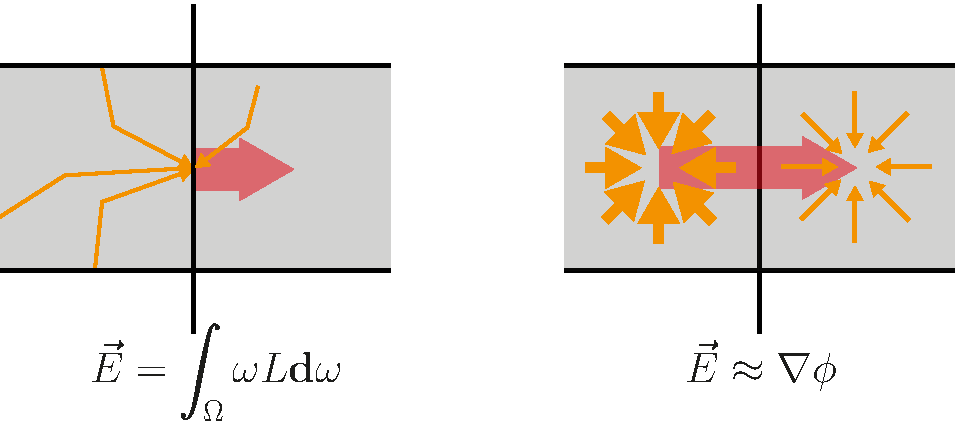
\includegraphics[width=0.85\textwidth]{05_diffusion_approximation/figures/fig_diffusion_idea.pdf}
\caption{Ficks first law of diffusion (visualized on the right) states that the diffusive flux can be related to the difference in concentration (of fluence $\phi$), allowing to approximate a global quantity (left) by a local quantity. This is the fundamental idea behind diffusion approximation.}
\label{fig:da_moment_problem_flux_as_fluence_gradient}
\end{figure}
The problem is now uniquely defined and can be solved with standard solvers. In the next section, we discuss how results from diffusion approximation compare against the results from the $P_N$-method.

\section{Diffusion Approximation}

\label{sec:diffusion_approximation}

The previous section derived a diffusion equation from the $P_1$-equations by assuming an isotropic distribution of the radiance field for the moment closure problem. We solve this diffusion equation very efficiently using a multigrid solver similarly to Stam et al.~\cite{Stam95} and discuss the results in this section.

The multigrid solver is implemented in straightforward fashion. However, since Stam only mentiones the use of a multigrid solver very briefly, we give more details on its implementation in appendix~\ref{sec:da_solver}.

In terms of the rendering integration, it is important to note that the diffusion approximation only gives the solution to the zero moment $L^{0,0}$, which is the same as the fluence $\phi$. Higher moments are not needed, if the phase function is isotropic, as discussed in section~\ref{sec:pn_rendering_integration} and shown in equation~\ref{eq:pn_rendering_integration2}. However, in case of an anisotropic phase function, equation~\ref{eq:pn_rendering_integration2} applies, which requires evaluation of $\widehat{L}_m$, the full reconstruction of the truncated spherical harmonics expansion of the radiance field. For the diffusion approximation this was derived in section~\ref{sec:da_moment_expansion_L} and resulted in equation~\ref{eq:moment_expansion_L}. While the first term is straightforward to evaluate using the zero moment from the diffusion solve, the second term requires the flux vector. This needs first to be computed using the definition, which had been derived using the isotropic moment closure in section~\ref{sec:moment_closure}, where equation~\ref{eq:diffusion_ficks_law} is used. With the definition, the first moment can be reconstructed from the gradient of the zero moment and used to evaluate $\widehat{L}_m$.

\subsection{Point Source Problem}
\label{sec:da_results_pointsource}
The solver is first run on the point source problem described in section~\ref{sec:pn_results_pointsource} and compared against the results from the $P_N$-method.
\begin{figure}[h]
\centering
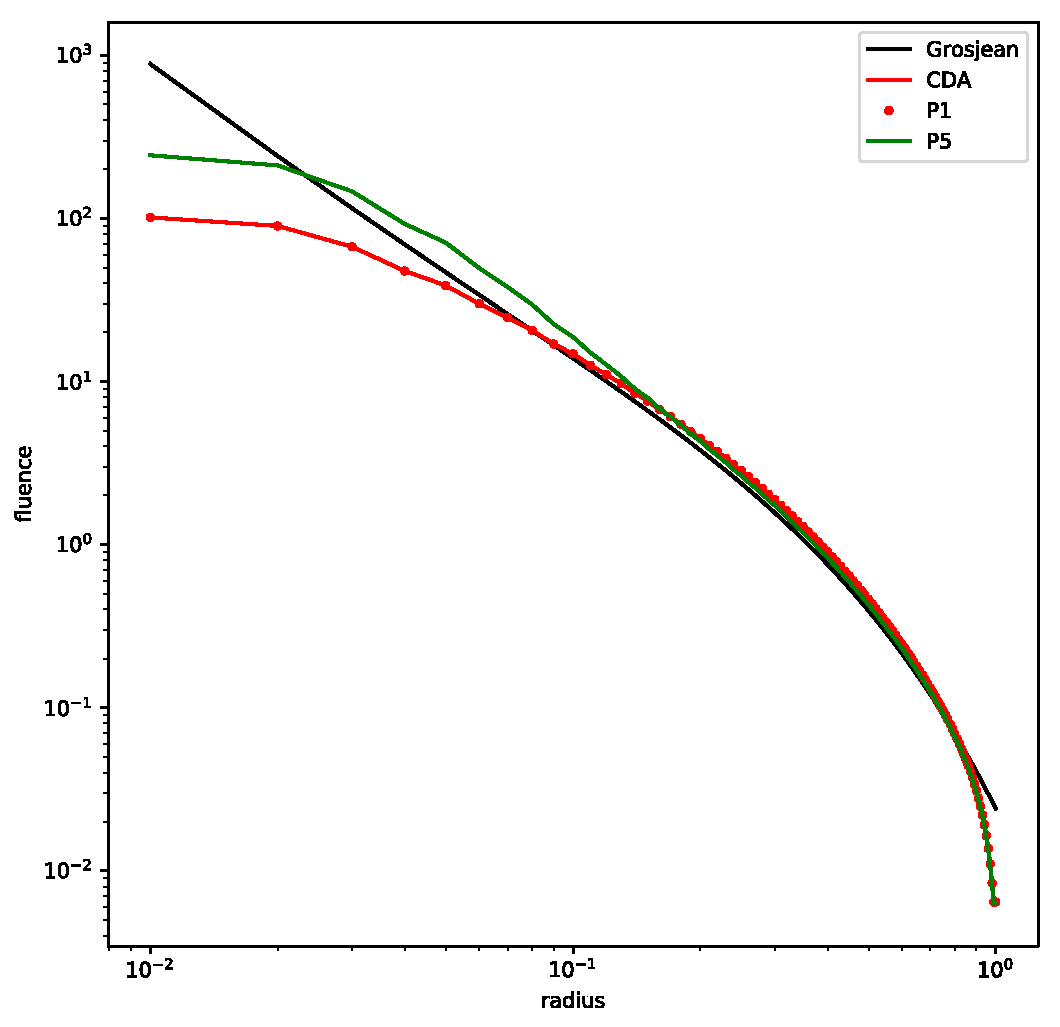
\includegraphics[width=0.8\textwidth]{05_diffusion_approximation/results/cda_result_plot_pointsource.pdf}
%\missingfigure{pointsource plots DA}
\caption{Solution of the diffusion approximation for the point source problem (red line) compared against ground truth (black), $P_1$ (red dots) and $P_5$~(green).}
\label{fig:da_results_pointsource_1}
\end{figure}

As expected, the accuracy of the $P_N$-result is better than for the diffusion approximation as soon as the truncation order of the $P_N$-method is increased. However, for truncation order of $N=1$, identical results are shown. This is explained by the fact that the diffusion approximation is derived by collapsing the $P_1$ equations by using substitution. Therefore, the diffusion equation is mathematically equivalent to the $P_1$-equations and consequently is satisfied by the exact same solution. This result further validates that the $P_N$-solver has been implemented correctly.


\begin{figure}[h]
\centering
\begin{subfigure}[t]{0.48\columnwidth}
\includegraphics[width=\columnwidth]{04_pn_method/results/nebulae_ms_groundtruth.png}
\caption{Pathtraced}
\label{fig:pn_results_nebulae1_pathtraced}
\end{subfigure}
\hspace{0.01\columnwidth}
\begin{subfigure}[t]{0.48\columnwidth}
\includegraphics[width=\columnwidth]{05_diffusion_approximation/results/nebulae_ms_cda.png}
\caption{Diffusion Approximation}
\label{fig:pn_results_nebulae1_P1}
\end{subfigure}

\begin{subfigure}[t]{0.48\columnwidth}
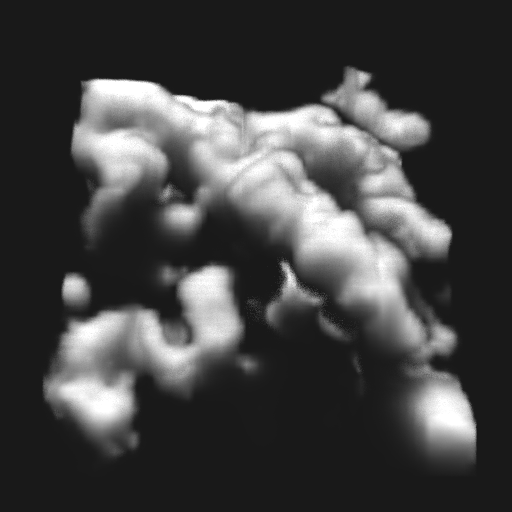
\includegraphics[width=\columnwidth]{04_pn_method/results/nebulae_p1_ms.png}
\caption{$P_1$}
\label{fig:pn_results_nebulae1_P3}
\end{subfigure}%
\hspace{0.01\columnwidth}
\begin{subfigure}[t]{0.48\columnwidth}
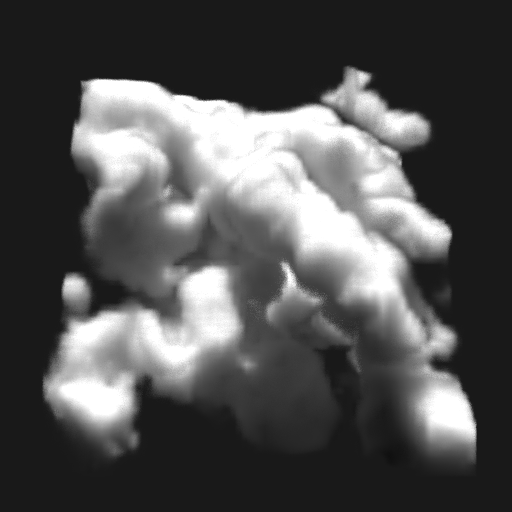
\includegraphics[width=\columnwidth]{04_pn_method/results/nebulae_p5_ms.png}
\caption{$P_5$}
\label{fig:pn_results_nebulae1_P5}
\end{subfigure}

%\vspace{-0.2in}
\caption{Diffusion approximation results for the procedural cloud dataset (multiple scattered light) compared against Monte-Carlo reference, $P_1$ and $P_2$.}
\label{fig:da_results_nebulae_1}
\end{figure}

\subsection{Procedural Cloud}
\label{sec:da_results_clouds}

Finally, the multigrid solver for diffusion is run on the procedural cloud problem from section~\ref{sec:pn_results_clouds}. The presence of vacuum regions in the dataset caused the $P_N$-method to not convergence, but it was still possible to run iterations that would reduce the residual error albeit slowly. However, for the diffusion approximation, the presence of vacuum regions causes the method to break down completely, as the diffusion coefficient (equation~\ref{eq:da_D}) requires division by the extinction coefficient and therefore produces a division by zero. This aspect is easily confused, when reading the neutron transport literature. Papers such as Hansen et al.~\cite{Hansen14} state that the normal form of the $P_N$-equations can deal with voids. This is true in the sense that it does not produce a division by zero directly. However, it still is not convergent.

As with the point source problem, it is shown that the $P_1$-results, match the diffusion results while higher truncation order produces more accurate results for the $P_N$-method. In particular, the diffusion approximation (or $P_1$) fail to reproduce the illumination of the indirectly illuminated region at the bottom of the dataset.
%\begin{figure}[h]
%\centering
%\missingfigure{procedural cloud convergence plots DA P1 P5}
%\caption{TODO}
%\label{fig:da_results_nebulae_2}
%\end{figure}


\section{Moment Problem Revisited}
\label{sec:moment_problem_revisited}

In section~\ref{sec:moment_closure}, it was established that a choice for the second moment of the radiance distribution was required to close the system of equations, which was found by collapsing the moment expansion of the radiative transfer equation, truncated after the first moment. The classical diffusion approximation was derived by assuming an isotropic radiance distribution for the second moment. In this section, we will take a closer look at the moments and carve out an important feature, which explains the bad accuracy of classical diffusion approximation in certain scenarios.

The distribution of power $\phi$ over solid angle was given by the normalized radiance $\widehat{L}$. Since it is a probability distribution, it has to integrate to one, which is easily verified
\begin{align*}
\int_{\Omega}{\hat{L}(\vec{x}, \omega)\ud\omega}=
\int_{\Omega}{\frac{L\left(\vec{x}, \omega\right)}{\phi\left(\vec{x}\right)}\ud\omega}=
\frac{1}{\phi\left(\vec{x}\right)}
\int_{\Omega}{L\left(\vec{x}, \omega\right)\ud\omega}
=1
=\hat{L}_0
\end{align*}
Further, we have that the normalized radiance $\widehat{L}$ has to be non-negative, in order to be a probability distribution:
\begin{align*}
\hat{L}(\vec{x}, \omega)\ge 0 \qquad \text{for all unit directions } \omega
\end{align*}
which is easily verified from the fact, that the radiance field is non-negative by definition:
\begin{align*}
L\left(\vec{x}, \omega\right) \ge 0
\implies
\int_{\Omega}{L(\vec{x}, \omega)\ud\omega}=\phi\left(\vec{x}\right)\ge 0
\implies
\frac{L\left(\vec{x}, \omega\right)}{\phi\left(\vec{x}\right)}=\widehat{L}(\vec{x}, \omega) \ge 0
\end{align*}

Akhiezer~\cite{Akhiezer65} established, that the probability distribution contraints on a function results in a set of inequalities between moments of this function. In particular, the non-negativity constraint on the radiance field $L$ and its normalized distribution impose a constraint between the zero moment and the first moment. In case of the radiance field, this constraint can be derived by considering the dot product between direction vectors $\omega'$ and $\omega$, both of unit length. We have
\begin{align*}
-1 \le \omega'\cdot\omega \le 1
\implies
0 \le 1 - \omega'\cdot\omega \le 1
\implies
\int_{\Omega}{\left(1-\omega'\cdot\omega\right)L\left(\vec{x}, \omega\right)\ud\omega}\ge 0
\end{align*}
which can be rearranged into
\begin{align*}
\int_{\Omega}{\left(1-\omega'\cdot\omega\right)L\left(\vec{x}, \omega\right)\ud\omega} &\ge 0
\\
\int_{\Omega}{L\left(\vec{x}, \omega\right)\ud\omega}
-\int_{\Omega}{\omega'\cdot\omega L\left(\vec{x}, \omega\right)\ud\omega}
&\ge 0
\\
\int_{\Omega}{L\left(\vec{x}, \omega\right)\ud\omega}
-\omega'\cdot\int_{\Omega}{L\left(\vec{x}, \omega\right)\omega\ud\omega}
&\ge 0
\\
\phi\left(\vec{x}\right)
-\norm{\vec{E}\left(\vec{x}\right)}
&\ge 0
\\
\phi\left(\vec{x}\right)
&\ge \norm{\vec{E}\left(\vec{x}\right)}
\end{align*}
This constraint states, that the total power at position $\vec{x}$ must never exceed the length of the flux-vector.
\TD{intuition behind flux-limit}

A very similar constraint can be derived for the normalized radiance $\widehat{L}$, by following the same steps above. This results in
\begin{align}
\label{eq:fld_flux_limit}
1
\ge
\norm{
\frac{\vec{E}\left(\vec{x}\right)}{\phi\left(\vec{x}\right)}
}
\end{align}
In the case of the classical diffusion approximation, we have $\vec{E}\approx-D\nabla\phi$ (equation~\ref{eq:diffusion_ficks_law}). Inserting this into equation~\ref{eq:fld_flux_limit} gives
\begin{align}
\label{eq:fld_flux_limit}
1
\ge
\norm{
\frac{\nabla\phi\left(\vec{x}\right)}{3\sigma_t\left(\vec{x}\right)\phi\left(\vec{x}\right)}
}
\end{align}
Here it can be seen clearly, that with the classical diffusion approximation, this constraint can be violated when the extinction coeffient $\sigma_t$ becomes very small, meaning in the presence of very thin medium. It breaks down completely in case of vacuum $\sigma_t=0$. The constraint can also be violated if the the fluence gradient becomes very large in relation to $\sigma_t\phi$. This happens very close to point light sources and near strong density gradients in the medium.

\todo[inline]{give intuition how the assumption of isotropic radiance distribution for the 2nd order tensor of the radiance field is violated strongly near boundaries or transitions from low to high density medium}

Violation of the constraint above means, that for the classical diffusion approximation, the flux vector is much larger than what is physically possible. Since the flux vector governs light transport, the literature often referres to classical diffusion as suffering from unphysical fluxes or unphysical light transport.


\subsubsection*{A Transport Regime Measure}

The right hand side of equation~\ref{eq:fld_flux_limit} is an important measure, which allows us to detect at every point within the domain, where and to what extend the diffusion approximation fails. And for this, only local information about the moments and extinction coefficient is needed. It is an important building block for the technique presented in this chapter, which seeks to improve the accuracy of the diffusion approximation.

The flux-limit in equation~\ref{eq:fld_flux_limit} can be factorized to make its intuition more clear:
\begin{align}
\label{eq:flux_limit_factors}
\norm{
\frac{\nabla\phi\left(\vec{x}\right)}{3\sigma_t\left(\vec{x}\right)\phi\left(\vec{x}\right)}
}
=
\frac{1}{3}
l\left(\vec{x}\right)
\frac{\norm{\nabla\phi\left(\vec{x}\right)}}{\phi\left(\vec{x}\right)}
\end{align}
It consists of two factors, of which the first is the mean free path $l$, which is the inverse of the extinction coefficient and therefore parameterizes the medium. If the mean free path is small and approaches zero, we know that photons travel only very short distances in average, before they encounter another interaction with the medium. In this case the medium is very dense. If the mean free path is large, the medium is very thin and photons travel long distances before they encounter another interaction with the medium. In case of vacuum, where no medium is present, photons travel unhindered and never interact. In this case the mean free path is infinite.
\missingfigure{transport regimes according to mean free path}
The second factor in equation~\ref{eq:flux_limit_factors} is the ratio between the length of the flux-vector (according to diffusion) and the zero moment. If the magnitude of the flux-vector is small, while the total power $\phi$ is large, we can infer that the incoming radiance is distributed equally over solid angle, which means that light is coming uniformly from all directions. If the flux-vector magnitude is large in comparison to the total power, we can infer that the energy is concentrating in certain directions. In the extreme case, when the total power is equal to the flux-vector magnitude, the light comes only from a single direction.
\missingfigure{transport regimes according to moment ratio}
The two factors in equation~\ref{eq:flux_limit_factors} parameterize the transport regime according to the medium and the distribution of incoming light over solid angle respectively. Combined, they are a local measure for the transport regime in general (as perceived by diffusion). If the medium is very dense (small mean free path) and light arrives equally distributed from all directions (small moment ratio), diffusive transport is dominating and the flux-limit is not violated. The diffusion approximation is a good approximation in these scenarios. If the medium is very thin (large mean free path) and the moment ratio approaches one, we have ballistic transport and free streaming in the case of vacuum or when the ratio is exactly one.

We ignore the $1/3$ factor in equation~\ref{eq:flux_limit_factors} and introduce $R$, a transport measure according to the diffusion approximation:
\begin{align}
R\left(\vec{x}\right)
= 
\frac{\norm{\nabla\phi\left(\vec{x}\right)}}{\sigma_t\left(\vec{x}\right)\phi\left(\vec{x}\right)}
\qquad
\qquad
\begin{array}{cc}
R\left(\vec{x}\right)\rightarrow 0 : \text{diffussive transport}\\
R\left(\vec{x}\right)\rightarrow 1 : \text{streaming transport}
\end{array}
\end{align}
In section~\ref{sec:moment_closure}, the diffusion approximation was derived by assuming isotropic distribution of radiance and therefore we see the same requirement in the fux-limit contraint, where a small moment ratio is required and implies, that light is arriving equally from all directions.

The idea of flux-limited diffusion is to avoid violation of the fux-limit and consquently prevent unphysical transport. The key idea behind flux-limited diffusion is to not only assume isotropic distribution, but also allow streaming transport and use the measure $R$, to locally realize the right mix between diffusive and streaming transport. The next important building block is therefore the question of how the diffusion equation looks like in the presence of streaming transport. This is outlined in the next section. Section~\ref{sec:fld_vef} will then develop flux-limited diffusion as a combination with classical diffusion.

\section{Streaming Limit Approximation}
\label{sec:fld_streaming_limit_approximation}

In the previous section, the transport measure $R$ was introduced, which contains the factor $\norm{\nabla\phi}/\phi$. This factor approaches one as transport becomes less diffusive and enters the streaming regime. In the case of $\norm{\nabla\phi}/\phi=1$, the length of the flux-vector matches the amount of total power. In this case, light is coming from a single direction. The radiance distribution of this configuration is given as
\begin{align}
\hat{L}\left(\omega\right)=\delta_{\Omega}\left(\omega,\vec{n}\right).
\end{align}
where $\delta_{\Omega}$ is the angular Dirac delta distribution into direction $\vec{n}$. Spatial dependency is omitted and not relevant for this discussion. The moments of this distribution are:
\begin{align}
\label{eq:zero_moment_Lhat}
\hat{L}_0\left(\omega\right)&=\int_{\Omega}{\delta_{\Omega}\left(\omega,\vec{n}\right)\ud\omega} = 1\\
\label{eq:first_moment_Lhat}
\hat{L}_1\left(\omega\right)&=\int_{\Omega}{\delta_{\Omega}\left(\omega,\vec{n}\right)\omega\ud\omega} = \vec{n}\\
\label{eq:second_moment_Lhat}
\hat{L}_2\left(\omega\right)&=\int_{\Omega}{\delta_{\Omega}\left(\omega,\vec{n}\right)\omega_i\omega_j\ud\omega} = \vec{n}_i\vec{n}_j
\end{align}
The zero moment expresses that all power given by $\phi$ comes from a single direction. The second equation shows, that the first moment of a delta distribution is identical to the vector which defines that distribution ($\vec{n}$ in our case). It shall be concluded that the length of the flux-vector equals the zero moment and its direction is $\vec{n}$ (all under the assumption of a delta radiance distribution):
\begin{align}
\label{eq:iso_delta_normE}
\vec{E} = \hat{L}_1\phi = \vec{n}\phi  &\implies \norm{\vec{E}} = \phi\\
&\implies \vec{E} \parallel \vec{n} \qquad \text{($\vec{E}$ and $\vec{n}$ are parallel)}
\end{align}
The second moment equation shows that the second moment is found by the outer product of the defining vector. Therefore, assuming a delta distribution results in the following Eddington tensor (equation~\ref{eq:eddington_tensor}):
\begin{align}
T_{ij} = \vec{n}_i\vec{n}_j
\label{eq:iso_delta_T}
\end{align}
The form of the Eddington tensor for a delta distribution of radiance in angular domain is given. In the end, this tensor is to be used to approximate the second moment of the radiance field $P$ in equation~\ref{eq:general_diffusion_equation} by $T\phi\approx P$. However, this way the direction $\vec{n}$ is introduced as another unknown. The next step in the derivation is, to reformulate $T$ and eliminate of the unknown $\vec{n}$, which is possible under certain assumptions.
%An important consideration is the fact, that the vector $\vec{n}$ is scaled to infinite length under the integral sign.
% \emph{This means our delta distribution is represented by a single vector of infinite length with direction $\vec{n}$}.

Inserting the approximation $T\phi$ into the flux-vector definition (equation~\ref{eq:me_first_resolved_E}) and assuming an isotropic emission $Q$ gives:
\begin{align*}
\vec{E}&= -\frac{1}{\sigma_t'}\operatorname{div}\left (T\phi\right )
\end{align*}
The key assumption used is that the spatial variations of $T$ can be neglected. Fundamentaly, the approach is to assume, that the radiance field $L$ can be separated into a product of two functions. One depending on angle and another function depending on position. This allows to express the divergence of the second moment as a matrix product with a gradient vector:
\begin{align}
\vec{E}&= -T\left(\frac{1}{\sigma_t'}\nabla\phi\right )
\label{eq:second_moment_iso2}
\end{align}
For the derivation the normalized flux will be addressed, which is given by scaling the flux-vector with $1/\phi$:
\begin{align}
\widehat{\vec{E}} = \frac{\vec{E}}{\phi}= -T\underbrace{\left(\frac{\nabla\phi}{\sigma_t'\phi}\right )}_{=\vec{R}}
\label{eq:second_moment_iso3}
\end{align}
Equation~\ref{eq:first_moment_Lhat} showed, that $\vec{n}$ points into the same direction as the flux-vector $\vec{E}$. This means, that the result of the transformation $T$ will be a vector, which is parallel to $\vec{n}$. Since the Eddington tensor has been constructed with $T_{ij}=\vec{n}_i\vec{n}_j$, it is known that $\vec{n}$ is the only eigenvector of $T$, with an eigenvalue greater than zero. It can be concluded that (under the assumption of negligible spatial variation of $T$) the transformation $T$ is applying a scaling operation and the dimensionless gradient $\vec{R}$ is parallel to $E$. Therefore the product of tensor $T$ is expressed with $\vec{R}$ as a scaling operation and equation~\ref{eq:second_moment_iso3} then becomes:
\begin{align}
\widehat{\vec{E}} = -\lambda\left(\frac{\nabla\phi}{\sigma_t'\phi}\right )
\label{eq:second_moment_iso4}
\end{align}
With an assumption about the spatial variation of $T$, the normalized flux-vector $\hat{L}_1$ could be expressed with respect to the zero moment $\phi$ and its spatial derivatives. What remains to be done is to find an expression for the eigenvalue $\lambda$. Then an expression for $\vec{E}$ (by using $\vec{E}=\hat{L}_1\phi$) would be found, which does not depend on itsself in anyway and therefore can be used to substitute $\vec{E}$ into the zero moment equation.

Apparently, finding $\lambda$ is easy in the case of a delta distribution of radiance. In that case it is known from equation~\ref{eq:iso_delta_normE}, that $\norm{\vec{E}}=\phi$ and therefore $\norm{\vec{E}/\phi}=1$. This requires that:
\begin{align*}
%\norm[\big]{\vec{f}}=\norm[\Bigg]
\norm{\vec{E}}
=
\norm{-\lambda\left(\frac{\nabla\phi}{\sigma_t'\phi}\right )}=1
\implies
\lambda=\frac{\sigma_t'\phi}{\norm{\nabla\phi}}
\end{align*}
Note that lambda is under the vector norm, which would make the sign of lambda ambiguous (it could be positive or negative: in both cases the length of the normalized flux-vector would be one). However, as mentioned earlier, the way $T=\vec{n}_i\vec{n}_j$ is defined allows the conclusion that $\lambda$ is the only Eigenvalue of $T$ and must be greater one. This gives the final expression for the flux-vector $\vec{E}$:
\begin{align*}
\vec{E}=\widehat{\vec{E}}\phi= -\lambda\left(\frac{\nabla\phi}{\sigma_t'\phi}\right )\phi= -\frac{\nabla\phi}{\norm{\nabla\phi}}\phi
,
\end{align*}
which states that the flux-vector is the unit vector pointing into the direction of the gradient of $\phi$ scaled by $\phi$ itself. Inserting this into the collapsed $P_1$-equation (equation~\ref{eq:general_diffusion_equation}) gives:
\begin{align}
\label{eq:iso_delta_advection_equation}
\nabla\cdot\left(\frac{\nabla\phi}{\norm{\nabla\phi}}\phi\right) &= \sigma_a\phi - Q_0
\end{align}
In case of a delta distribution of radiance in angular domain and with the assumption of negligible spatial variation of $T$, the moment equation turns into an advection equation, where the zero moment quantity $\phi$ is moved around by its normalized gradient.

This section highlights that the streaming transport is best represented by advection in case of the two term expansion of the radiative transfer equations. The core idea behind flux-limited diffusion is, to mix diffusive transport and advective transport, depending on local properties at $\vec{x}$. This is developed in the next section.
\section{The Variable Eddington Factor}
\label{sec:fld_vef}

In the two previous sections, diffusion theories have been derived for the two extreme limits of transport. That is purely isotropic radiance, which happens in the limit of thick, highly scattering media or a delta distribution, which in turn happens in the limit of very transparent, low order scattering media. This section will introduce the variable Eddington Factor, which has its origins in the astrophysics domain (Brunner~\cite{Brunner02}). It serves as a conceptual framework in which flux-limited diffusion is embedded. While diffusive transport has been related to a diffusion equation, the streaming transport has been shown to relate to advection. The Variable Eddington Factor allows to realize and mix both types of transport within a domain.
\begin{figure}[h]
\centering
%\missingfigure{show advection and diffusion transport}
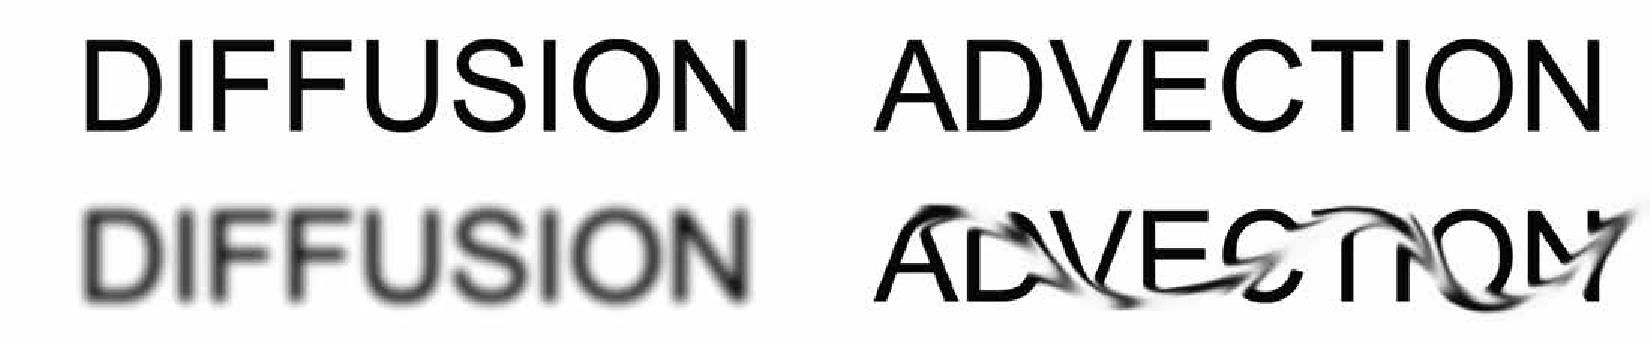
\includegraphics[width=0.95\textwidth]{06_fld/figures/fig_diffusion_vs_advection.pdf}
\caption{Illustration of diffusive (left) and advective (right) transport of particles. With diffusion, particles spread locally depending on the gradient of the particle distribution, which for flux-limited diffusion is the zero moment, the fluence. Advection is the movement of particles along a directed force field. For flux-limited diffusion, this force field is defined by the first moment, the flux vector.}
\label{fig:fld_vef_advection_diffusion}
\end{figure}


Classical diffusion assumed an isotropic distribution of radiance for the second moment, while pure streaming transport assumed a delta distribution. The Variable Eddington Factor theory assumes a radiance distribution, which is rotationally symmetric around a dominant vector $\vec{n}$. This assumption allows to derive a form for $T$, which represents isotropic distribution as well as a pure delta distribution and those forms inbetween, which are rotationally symmetric around a dominant direction $\vec{x}$.
\begin{figure}[h]
\centering
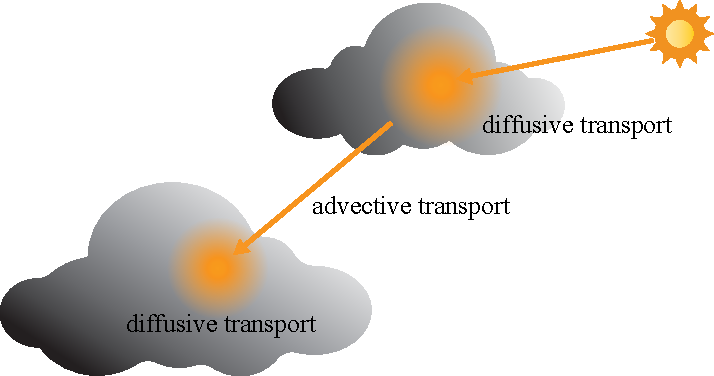
\includegraphics[width=0.55\textwidth]{06_fld/figures/fig_transport_regimes_scene.pdf}
%\missingfigure{show image with isotropic distribution, streaming limit distribution and inbetween forms}
\caption{Radiative transfer in typical scenes contains a mix of transport regimes as shown in this figure. Diffuse transport in dense media with high absorption and advective transport in thin media. The idea behind the Variable Eddington Factor is to express radiative transfer as a mix between those two extreme transport modes.}
\label{fig:fld_vef_advection_diffusion2}
\end{figure}

The Variable Eddington Factor form of $T$ is derived by considering a principal direction of transport, given by the vector $\vec{n}$ of unit length. An important assumption is that the radiance distribution will be radially symmetric around this direction. This means, that the value of $\hat{L}$ will be invariant to a rotation about axis $\vec{n}$. It follows, that its first and second moment $\hat{L}_1$ and $\hat{L}_2$ will also be invariant to rotation about $\vec{n}$. If one approximates $\hat{L}_2$ using the Eddington tensor $T$ with $\hat{L}_2\approx T\phi$, it can be concluded that $\vec{n}$ will be an eigenvector of $T$ with eigenvalue $\chi$:
\begin{align*}
T\vec{n} = \chi\vec{n}
\end{align*}
%\TD{explain/give reference why eigenvectors need to sum up to one}
The plane perpendicular to $\vec{n}$ is an eigenspace of $T$. By requiring that all eigenvalues sum up to one, the eigenvalues of the two eigenvectors spanning that plane by distributing the remaining eigenvalue $1-\chi$ evenly between both is expressed as:
\begin{align}
\frac{1}{2}\left(1-\chi\right)\mathbf{I}
\label{eq:iso_var_T_isoterm}
\end{align}
From the free streaming limit case (section~\ref{sec:fld_streaming_limit_approximation}), it is known that $\chi=1$, when the radiance distribution becomes a delta distribution (equation~\ref{eq:zero_moment_Lhat} and~\ref{eq:first_moment_Lhat}). In that case, the eigenvalues associated with the eigenvectors perpendicular to $\vec{n}$ become zero and the term above vanishes.

Tensor diagonalization allows to explicitly add the eigenvector $\vec{n}$ by adding the matrix $\vec{n}_i\vec{n}_j$ (with $\vec{n}$ being of unit length). The scaling of its coefficients is found by considering that the term in equation~\ref{eq:iso_var_T_isoterm} introduces three eigenvectors. The sum of their eigenvalues will be $3/2(1-\chi)$. Since eigenvalues of the final tensor $T$ need to add up to one, the eigenvalue associated with the matrix $\vec{n}_i\vec{n}_j$ will be $\left(1- \frac{3}{2}\left(1 - \chi\right)\right)$. This results in the following form for $T$:
\begin{align}
T &= \frac{1}{2}\left(1-\chi\right)\mathbf{I} + \left(1- \frac{3}{2}\left(1 - \chi\right)\right) \vec{n}\otimes\vec{n}
\nonumber
\\
&= \frac{1}{2}\left(1-\chi\right)\mathbf{I} + \frac{1}{2}\left(3\chi-1\right) \vec{n}\otimes\vec{n}
\label{eq:iso_var_T}
\end{align}
This form of $T$ is called the Variable Eddington Tensor (VET). It can be understood as an \emph{interpolation} between an isotropic distribution tensor ($1/3\mathbf{I}$) and a delta distribution tensor ($\vec{n}_i\vec{n}_j$). The variable $1/3 \le \chi \le 1$ is the interpolation variable and is called the Eddington factor (VEF). Theories, which respect this structure of the Eddington tensor are referred to as theories under the variable Eddington factor formalism (VEF-formalism).

If $\chi=1/3$, then equation~\ref{eq:iso_var_T} will result in the isotropic distribution tensor, which is the base assumption for classical diffusion:
\begin{align}
\frac{1}{2}\frac{2}{3}\mathbf{I} + \frac{1}{2}\left(\frac{3}{3}-1\right) \vec{n}\otimes\vec{n}
=\frac{1}{3}\mathbf{I} + 0\vec{n}\otimes\vec{n} = \frac{1}{3}\mathbf{I}
\end{align}
For $\chi=1$, equation~\ref{eq:iso_var_T} produces the Eddington tensor, which was derived for the pure streaming limit distribution, where all light comes from a singular direction:
\begin{align}
\frac{1}{2}0\mathbf{I} + \vec{n}\otimes\vec{n}
= \vec{n}\otimes\vec{n}
\end{align}
The Eddington factor $\chi$ can also be interpreted as a measure of anisotropy of the radiance distribution $\widehat{L}$ with respect to direction $\vec{n}$. It can be expressed in terms of the radiance distribution by the squared mean cosine (given by Levermore~\cite{Levermore84}):
\begin{align}
\chi &= \int_{S^2}{ \left(\omega\cdot\vec{n}\right)^2\hat{L}\left(\vec{x}, \omega\right)\ud\omega}
\label{eq:iso_var_chi}
\end{align}
With the variable Eddington factor approach, only a function for the interpolation variable $\chi$ (the actual Eddington factor) needs to be identified. This function should have $1/3$ and $1$ as its limits. With such an interpolation function, the limit transport cases (diffusion and free streaming) will be a subset of any theory, which adheres to the variable Eddington factor concept.

The Eddington factor framework, sets up the Eddington factor and the limits of its parameterization, $\chi$. The specific expression for this factor is not defined and it is clear that there are many options for the function $\chi$, which respect the given function limits. This is why there is such a rich variety of theories in other domains, which all propose their own version of that interpolation function. Some of them are ad-hoc schemes (Bowers et al.~\cite{Bowers82}, Kershaw~\cite{Kershaw76} and Larsen et al.~\cite{Larsen74}), which are derived from heuristics, while others have a clear connection to transport theory (Levermore at al.~\cite{Levermore81}) or are derived from entropy theory (Minerbo~\cite{Minerbo78}).

The general strategy for all these different variable Eddington factor theories is:
\begin{enumerate}
\item Find a model or theory, from which a certain radially symmetric form of the radiance distribution $\hat{L}$ about the normalized flux-vector$\vec{E}/\phi$ can be found or justified.
\item Then derive an expression for $\chi(\vec{E}/\phi)$ from the model for $\hat{L}$, which can be used to construct $T$. Further assumptions are applied, to be able to express $\vec{E}$ in terms of $\nabla\phi$. This is required in order to not have $T$ depend on the flux-vector directly as it still needs to be possible to resolve equation~\ref{eq:me_first_resolved_E} for the flux-vector.
\end{enumerate}

In this thesis, results for different theories have been presented and implemented, but only flux-limited diffusion from Levermore et. al~\cite{Levermore81} was discussed, since it is the most popular and also has the strongest connection to transport theory. Discussing all other theories is beyond the scope of this thesis and also not really necessary, as it is shown in section~\ref{sec:fld_results} that the particular choice of theory is not of significant importance for applications in computer graphics.
\section{Flux-limiters}
\label{sec:fld_vef_factors}

Levermore et. al~\cite{Levermore81} construct their theory by starting from the time-dependent form of the radiative transfer equation. They further assume a constant phase function $f_p=1/(4\pi)$:
\begin{align}
\label{eq:iso_var_fld_rte}
\frac{1}{c}\frac{\partial (\phi\hat{L})}{\partial t} + \left(\vec{\omega}\cdot\nabla\right)(\phi\hat{L})&=-\sigma_t\phi\hat{L} + \frac{1}{4\pi}\sigma_s\phi + Q
\end{align}
After applying the moment expansion, for the first moment equations are as follows:
\begin{align}
\label{eq:iso_var_fld_rte_zero}
\frac{1}{c}\frac{\partial \phi}{\partial t} + \nabla\vec{E} &= -\sigma_a\phi + Q_0
\end{align}
As a next step, equation~\ref{eq:iso_var_fld_rte_zero} is resolved for $\partial \phi/\partial t$ on the left hand side and used to substitute $\partial\phi/\partial t$ in equation~\ref{eq:iso_var_fld_rte} (after applying the product rule to the time derivative term). By further assuming the absence of self-emission ($Q=0$) and that the space and time derivatives of the radiance distribution $\hat{L}$ can be neglected, the result is:
\begin{align}
\label{eq:iso_var_fld_eliminated_time}
\left( \left(\vec{\omega}\cdot\nabla\right)\phi -\vec{f}\cdot\nabla\phi + \sigma_t'\phi\right)\hat{L} = \frac{1}{4\pi}\sigma_t'\phi
\end{align}
Solving equation~\ref{eq:iso_var_fld_eliminated_time} for $\hat{L}$ gives:
\begin{align}
\label{eq:iso_var_fld_Lhat}
\hat{L} = \frac{1}{4\pi}\frac{1}{1+\widehat{\vec{E}}\cdot\vec{R}-\vec{\omega}\cdot\vec{R}}
\end{align}
with
\begin{align}
\label{eq:iso_var_fld_R}
\vec{R} = -\frac{\nabla\phi}{\sigma_t'\phi}
\end{align}
The definition of the flux-vector in equation~\ref{eq:second_moment_iso3} is used, which was derived in section~\ref{sec:fld_streaming_limit_approximation}:
\begin{align}
\widehat{\vec{E}} = \frac{\vec{E}}{\phi}= T\vec{R}
\label{eq:iso_var_fld_normalized_flux}
\end{align}

Following the same argument about the radial symmetry of $\hat{L}$ and its relation to the flux-vector and eigenvectors of $T$, $T$ is replaced with a proportionality function $\lambda(R)$, where $R=\norm{\vec{R}}$:
\begin{align}
\widehat{\vec{E}} = \lambda(R)\vec{R}
\label{eq:iso_var_fld_relation_normalized_flux_R}
\end{align}

Using this in equation~\ref{eq:iso_var_fld_Lhat} gives:
\begin{align}
\label{eq:iso_var_fld_Lhat_R}
\hat{L} = \frac{1}{4\pi}\frac{1}{1+\lambda(R)R^2-\vec{\omega}\cdot\vec{R}}
\end{align}

By enforcing that $\hat{L}$ integrates to one over the solid angle of the unit sphere, the following expression for $\lambda(R)$ can be derived:
\begin{align}
\label{eq:iso_var_fld_lambdaR}
\lambda(R) = \frac{1}{R}\left(\mathbf{\operatorname{coth}}R - \frac{1}{R}\right)
\end{align}

Using this result and equation~\ref{eq:iso_var_fld_relation_normalized_flux_R}, gives the following expression for the flux vector:
\begin{align}
\label{eq:iso_var_fld_fluxvector}
\vec{E} = \widehat{\vec{E}}\phi=-\frac{1}{\sigma_t'}\lambda(R)\nabla\phi
\end{align}

Inserting this into the zero moment equation (equation~\ref{eq:me_zero}) gives the flux-limited diffusion equation, a diffusion-type equation of the following form:
\begin{align}
\label{eq:iso_var_fld_final}
\nabla\left( \underbrace{-\frac{1}{\sigma_t'}\lambda(R)}_{D_F}\nabla\phi\right) &= -\sigma_a\phi + Q_0
\end{align}

The flux-limited diffusion coefficient $D_F$ is non-linear and therefore turns the zero moment equation into a non-linear diffusion equation. $\lambda(R)$ is called the flux-limiter. In the diffusion limit, $R$ approaches zero and the flux-limiter approaches $\lambda(R)=1/3$, which will turn equation~\ref{eq:iso_var_fld_final} into the classical diffusion equation for isotropic media.
\begin{align}
\lim_{R\rightarrow 0 }D_F =-\frac{1}{3\sigma_t'}
\implies
\nabla
\left(
-\frac{1}{3\sigma_t'\left(\vec{x}\right)}
\nabla \phi\left(\vec{x}\right)
\right)
=
-\phi(\vec{x})\sigma_a(\vec{x})
+Q_0\left(\vec{x}\right)
\end{align}
In the transport limit, $R$ will approach infinity and the diffusion coefficient will cause the equation to become an advection equation as seen in the delta radiance distribution case (equation~\ref{eq:iso_delta_advection_equation}):
\begin{align}
\lim_{R\rightarrow\infty }D_F =-\frac{\phi}{\norm{\nabla\phi}}
\implies
\nabla
\left(
-\phi\frac{\nabla\phi\left(\vec{x}\right)}{\norm{\nabla\phi}}
\right)
=
-\phi(\vec{x})\sigma_a(\vec{x})
+Q_0\left(\vec{x}\right)
\end{align}
It can be seen that the flux-limited diffusion coefficient will normalize the fluence gradient $\nabla\phi$ to unit length and scale with the total power $\phi$. Flux-limited diffusion not only suppresses the flux in the free streaming transport regime, it also saturates it at the appropriate value to ensure correct free propagation (at the level of the approximation).

The flux-limiter introduced by Levermore et al.~\cite{Levermore81} was shown to relate to the variable Eddington factor approach in a seperate study (\cite{Whalen82, Levermore84}) to be:
\begin{align}
\label{eq:iso_var_fld_vef}
\chi = \lambda(R) + \lambda(R)^2R^2
\end{align}
As mentioned in the previous section, the theory sets up the limits, which flux-limiters have to respect. This allows different models and theories to find and justify particular choices of flux-limiters. Table~\ref{tbl:flux-limiters} presents the most prominent flux-limiters.
\begin{table}[h]
\center
\caption{Various prominent flux-limiters which all respect the Eddington factor limits and represent different flux-limited diffusion theories.}
\begin{tabular}{ l l }
\hline\hline
 Flux-limiter & $\lambda\left(R\right)$ \\ 
\hline
 sum~\cite{Bowers82} & $(3+R)^{-1}$ \\
 max~\cite{Bowers82} & $\mbox{max}(3, R)^{-1}$ \\
 Kershaw~\cite{Kershaw76} & $2(3+\sqrt{9 + 4R^2}\,)^{-1}$ \\
 Larsen-$n$~\cite{Larsen74} & $(3^n + R^n)^{-\frac{1}{n}}$ \\
 Levermore-Pomraning~\cite{Levermore81} & $\frac{1}{R} \left(\coth(R)-\frac{1}{R}\right)$    
\end{tabular}
\label{tbl:flux-limiters}
\end{table}

\begin{figure}[h]
\centering
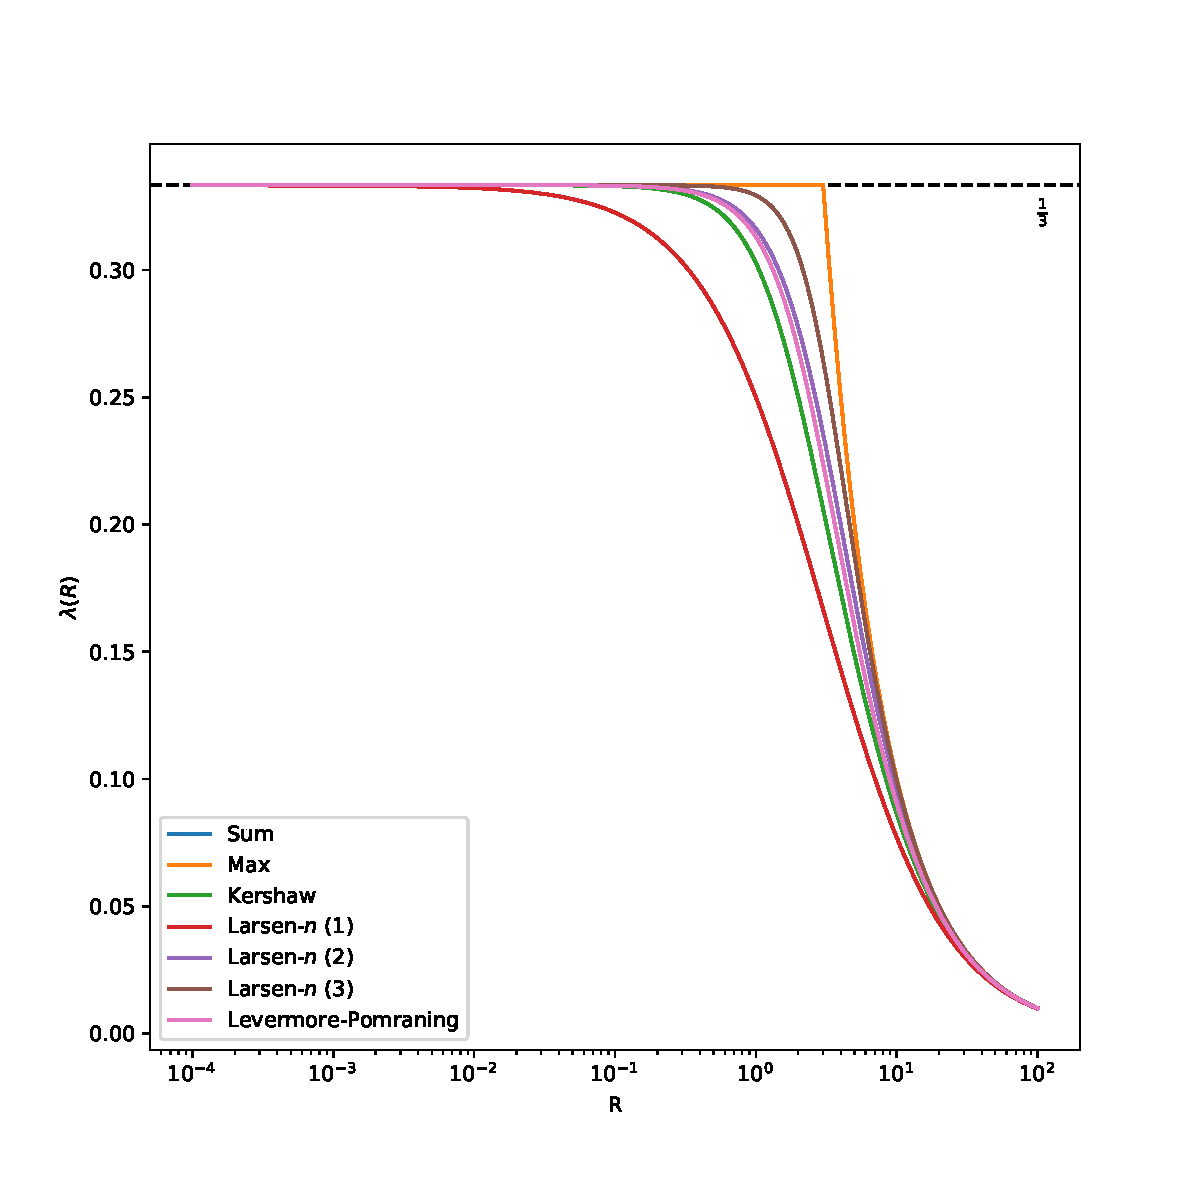
\includegraphics[width=0.65\textwidth]{06_fld/figures/plot_flux_limiters.pdf}
\caption{Plot of the various flux-limiters shown in table~\ref{tbl:flux-limiters}.}
\label{fig:flux-limiters}
\end{figure}
%
%\missingfigure{flux-limiters graphs}

In this section a non-linear form of the diffusion equation is derived which respects the flux-limit constraint. The following section will present a novel solver, which solves flux-limited diffusion on a finite difference grid over a given domain.

\section{Non-Linear Gauss-Seidel Solver with Successive Overrelaxation}
\label{sec:fld_solver}

In this section, a new method for solving the modified diffusion equation provided by flux-limited diffusion theory is introduced. Most prominent with the flux-limited diffusion equation is the non-linear diffusion coefficient. Unfortunately, this non-linearity prevents application of any components of the solver-framework that was developed in chapter~\ref{sec:pnmethod} and application of the multigrid solver developed in chapter~\ref{sec:diffusion_approximation}, as both are exclusively geared towards coupled systems of linear partial differential equations.

The equation, which has to be solved is the flux-limited diffusion equation (equation~\ref{eq:iso_var_fld_final}). The flux-limiter $\lambda$ by Levermore et al.~\cite{Levermore81} will be used (equation~\ref{eq:iso_var_fld_lambdaR}), which in term depends on the transport measure $R$ (equation~\ref{eq:fld_transport_measure_R}). In summary the solver developed in this section seeks out to find a solution for $\phi$, which satisfies the following set of equations:
\begin{align}
\nabla\left(D_F\left(\vec{x}\right)\nabla\phi\right) &= -\sigma_a\phi + Q_0
\quad \text{with}\quad
D_F\left(R\left(\vec{x}\right)\right) = -\frac{1}{\sigma_t'}\lambda\left(R\left(\vec{x}\right)\right)
\label{eq:fld_solver_diffusion_equation}
\\
\lambda(R\left(\vec{x}\right)) &= \frac{1}{R\left(\vec{x}\right)}\left(\mathbf{\operatorname{coth}}R\left(\vec{x}\right) - \frac{1}{R\left(\vec{x}\right)}\right)
\label{eq:fld_solver_flux_limiter}
\\
R\left(\vec{x}\right) &= \frac{\norm{\nabla\phi\left(\vec{x}\right)}}{\sigma_t\left(\vec{x}\right)\phi\left(\vec{x}\right)}
\label{eq:fld_solver_transport_measure_R}
\end{align}
This is a diffusion equation with a non-linear diffusion coefficient $D_F$ which depends on the flux-limiter $\lambda$. The non-linearity arises from the fact that the flux-limiter depends on the solution, which after substitution will create non-linear terms in the partial differential equation.

\subsubsection*{Discretization}

Discretizing equation~\ref{eq:fld_solver_diffusion_equation} using a finite difference grid is straightforward and results in the following partial differential equation:
\begin{align}
\frac{1}{h_x^2}D_{i-\frac{1}{2}}\phi_{i-1}
+\frac{1}{h_x^2}D_{i+\frac{1}{2}}\phi_{i+1}
+\frac{1}{h_y^2}D_{j-\frac{1}{2}}\phi_{j-1}
\\
+\frac{1}{h_y^2}D_{j+\frac{1}{2}}\phi_{j+1}
+\frac{1}{h_z^2}D_{k-\frac{1}{2}}\phi_{k-1}
+\frac{1}{h_z^2}D_{k+\frac{1}{2}}\phi_{k+1}
\\
-\left(
\frac{1}{h_x^2}D_{i-\frac{1}{2}}+\frac{1}{h_x^2}D_{i+\frac{1}{2}}
+\frac{1}{h_y^2}D_{j-\frac{1}{2}}+\frac{1}{h_y^2}D_{j+\frac{1}{2}}
+\frac{1}{h_z^2}D_{k-\frac{1}{2}}+\frac{1}{h_z^2}D_{k+\frac{1}{2}}
\right)
\phi_{ijk}
\\
= -\sigma_{a, ijk}\phi_{ijk} + q_{ijk}
\label{eq:fld_solver_discretized_diffusion_equation}
\end{align}
The subscript to the diffusion coefficient $D_F$ has been omitted for readability. Since it is defined at voxel centers, its off-center values are found by interpolation. For example,
\begin{align}
D_{i+\frac{1}{2}} = \frac{1}{2}\left( D_{i}+D_{i+1}\right)\ .
\label{eq:fld_solver_D_interpolated}
\end{align}
The flux-limiter in equation~\ref{eq:fld_solver_flux_limiter} is simply discretized by using the discretized transport measure $R_{ijk}$:
\begin{align}
\lambda(R_{ijk}) &= \frac{1}{R_{ijk}}\left(\mathbf{\operatorname{coth}}R_{ijk} - \frac{1}{R_{ijk}}\right)
\label{eq:fld_solver_discrete_flux_limiter}
\end{align}
Note that the transport measure $R$ will cause a division by zero if it becomes zero. This problem will be addressed by the way the transport measure $R$ in equation~\ref{eq:fld_solver_transport_measure_R} is discretized:
\begin{align}
R_{ijk} = \frac{\operatorname{max}\left(\norm{\nabla\phi_{ijk}},\epsilon\right)}{\operatorname{max}\left(\sigma_{t,ijk}\phi_{ijk},\epsilon\right)}
\quad
\text{with}
\quad
\nabla\phi_{ijk} = \frac{1}{2}
\left(
\begin{array}{c}
\frac{1}{h_x}\phi_{i+1}-\frac{1}{h_x}\phi_{i-1} \\
\frac{1}{h_y}\phi_{j+1}-\frac{1}{h_y}\phi_{j-1} \\
\frac{1}{h_z}\phi_{k+1}-\frac{1}{h_z}\phi_{k-1} \\
\end{array}
\right)
\label{eq:fld_solver_discrete_R}
\end{align}
The introduction of a minimum threshold $\epsilon$ in the nominator and denominator will prevent $R$ from becoming zero or breaking down due to division by zero. Note that the minimum threshold $\sigma_{min}$ of the extinction coefficient will be applied on top.


\subsubsection*{Non-linear Gauss-Seidel Solver}

The solver follows an iterative segregated approach for solving non-linear partial differential equations (Mazumder~\cite{Mazumder2015}). The idea is to update the diffusion coefficient from the current solution $\phi_{ijk}$ (initialized by an initial guess) and then update the solution using the updated diffusion coefficient values $D_{ijk}$ and repeat this update procedure until convergence to a final solution.

The iteration method used is the Gauss-Seidel fixpoint iteration scheme. The non-linearity is integrated by updating the diffusion coefficient in place during iteration over all voxels for a single Gauss-Seidel step.

The Gauss-Seidel update step is found by isolating $\phi_{ijk}$ in the discretized diffusion equation~\ref{eq:fld_solver_discretized_diffusion_equation}:
\begin{equation}
\label{eq:fld_solver_gs_phi_update}
\resizebox{1.0\hsize}{!}{$
\phi_{ijk} =
\\
\frac
{
\frac{1}{h_x^2}D_{i-\frac{1}{2}}\phi_{i-1}
+\frac{1}{h_x^2}D_{i+\frac{1}{2}}\phi_{i+1}
+\frac{1}{h_y^2}D_{j-\frac{1}{2}}\phi_{j-1}
+\frac{1}{h_y^2}D_{j+\frac{1}{2}}\phi_{j+1}
+\frac{1}{h_z^2}D_{k-\frac{1}{2}}\phi_{k-1}
+\frac{1}{h_z^2}D_{k+\frac{1}{2}}\phi_{k+1}
+q_{ijk}
}
{
-\left(
\frac{1}{h_x^2}D_{i-\frac{1}{2}}+\frac{1}{h_x^2}D_{i+\frac{1}{2}}
+\frac{1}{h_y^2}D_{j-\frac{1}{2}}+\frac{1}{h_y^2}D_{j+\frac{1}{2}}
+\frac{1}{h_z^2}D_{k-\frac{1}{2}}+\frac{1}{h_z^2}D_{k+\frac{1}{2}}
-\sigma_{a, ijk}
\right)
}
$}
\end{equation}
Then the discrete transport measure $R_{jk}$ is updated, using the newly retrieved value for $\phi_{ijk}$. With this the new diffusion coefficient is computed:
\begin{align}
D_{ijk} = \frac{\lambda\left(R_{ijk}\right)}{\sigma_t'}
\label{eq:fld_solver_discrete_D}
\end{align}
This update step is executed for every voxel of the finite difference grid and values are updated in place.

The values $\phi_{ijk}$ and $D_{ijk}$ are initialized to small tolerances $\phi_{ijk} = \epsilon \bar{j}\Delta l$ and $D_{ijk} = \epsilon \Delta l$ for all voxels. Initially, these grid values do not satisfy equation~\ref{eq:fld_solver_gs_phi_update} and equation~\ref{eq:fld_solver_discrete_D}, but over a number of iterations they converge to a consistent solution of both equations over the whole grid. 

Boundary conditions are accounted for by updating the values for $\phi_{ijk}$ and $D_{ijk}$ at the boundary voxels. For Dirichlet boundary conditions the values are set directly. For Neumann boundary conditions the boundary voxels are set according to the next inner voxel (section~\ref{sec:pn_bc}). This update is done at the beginning of each Gauss-Seidel iteration.

A criteria will decide when the algorithm ran enough Gauss-Seidel iterations. For real-time applications a specific user-decided number of iterations might be a reasonable choice. Here convergence to floating-point precision may be compromised to retain interactivity. Another option is to compute the root mean square of the residual and stop the Gauss-Seidel algorithm as soon as this falls below a user-defined threshold.

To improve the rate of convergence, successive over-relaxation (SOR) is used (Hadjidimos~\cite{Hadjidimos00}). Defining the over-relaxation parameter $\omega$, where $0<\omega<2$, the update of $\phi_{ijk}$ at each stencil is modified to:
\begin{equation}
\label{eq:fld_solver_sor_update}
\phi_{ijk} \leftarrow \omega \,\phi'_{ijk} + (1-\omega)\phi_{ijk} 
\end{equation}
where $\phi'_{ijk}$ is the updated value from equation~\ref{eq:fld_solver_gs_phi_update}.

To further speed up the computation time a Red-Black Gauss-Seidel update process is used. This allows to update half of the voxels in parallel (Olshanskii et al.~\cite{Olshanskii14}). The voxels are seperated into two disjunct groups according to a checkerboard pattern (hence the name Red-Black). Voxels within a group can be updated in parallel, because the stencil only requires information from the neighbouring voxels in each dimension and those always belong to the other voxel group. Firstly, all voxels of one group are processed in parallel and their $\phi_{ijk}$ and $D_{ijk}$ values are updated. Then all the voxels of the other group are updated in parallel. The two passes constitute one iteration. The full algorithm is outlined in listing~\ref{algorithm:fld_solver}.



\begin{algorithm}[!ht]
\caption{Non-linear Gauss-Seidel SOR FLD solver}
\begin{algorithmic}
\State Initialize voxel grids $\phi$, $D$
\Repeat
    \State Update boundary voxels
    \ParFor{all red non-boundary voxels $ijk$}
    \State Compute $R_{ijk}$ (equation~\ref{eq:fld_solver_discrete_R})
    \State Compute $\lambda\left(R_{ijk}\right)$ (equation~\ref{eq:fld_solver_discrete_flux_limiter})
    \State Compute and update $D_{ijk}$ (equation~\ref{eq:fld_solver_discrete_D})
    \State Compute $D_{i\pm\frac{1}{2}}$, $D_{j\pm\frac{1}{2}}$ and $D_{k\pm\frac{1}{2}}$ (according to equation~\ref{eq:fld_solver_D_interpolated})
    \State Compute $\phi_{ijk}'$ (equation~\ref{eq:fld_solver_gs_phi_update})
    \State Compute and update $\phi_{ijk}$ using equation~\ref{eq:fld_solver_sor_update}
    \EndParFor
    \ParFor{all black non-boundary voxels $ijk$}
    \State Same as above but just for the black voxels
    \EndParFor
    \State If required, compute root mean square of residual\;
\Until{convergence criteria is met}
\end{algorithmic}
\label{algorithm:fld_solver}
\end{algorithm}

\section{Results}
\label{sec:fld_results}

With the solver introduced in the previous section it can now be run for comparison on the problems, which were used for the $P_N$-method in chapter~\ref{sec:pnmethod} and the diffusion approximation in chapter~\ref{sec:diffusion_approximation}.

The rendering integration aspects to be considered are identical to the diffusion approximation (section~\ref{sec:da_results}). As with the diffusion approximation, flux-limited diffusion will give a solution for the zero moment $\phi$ from which the second moment can be recovered using equation~\ref{eq:diffusion_ficks_law}. Both moments can be used to reconstruct the truncated spherical harmonics expansion of the radiance field by using equation~\ref{eq:moment_expansion_L}. The difference to the diffusion approximation solution is that the fluence should be more accurate as the flux-limit constraint had been accounted for.

\subsection{Point Source Problem}
\label{sec:pn_results_pointsource}

At first it shall be turned towards the point source problem in order to validate the results from the flux-limited diffusion solver and assess its accuracy by comparing against an analytical ground truth solution.
\begin{figure}[h]
\centering
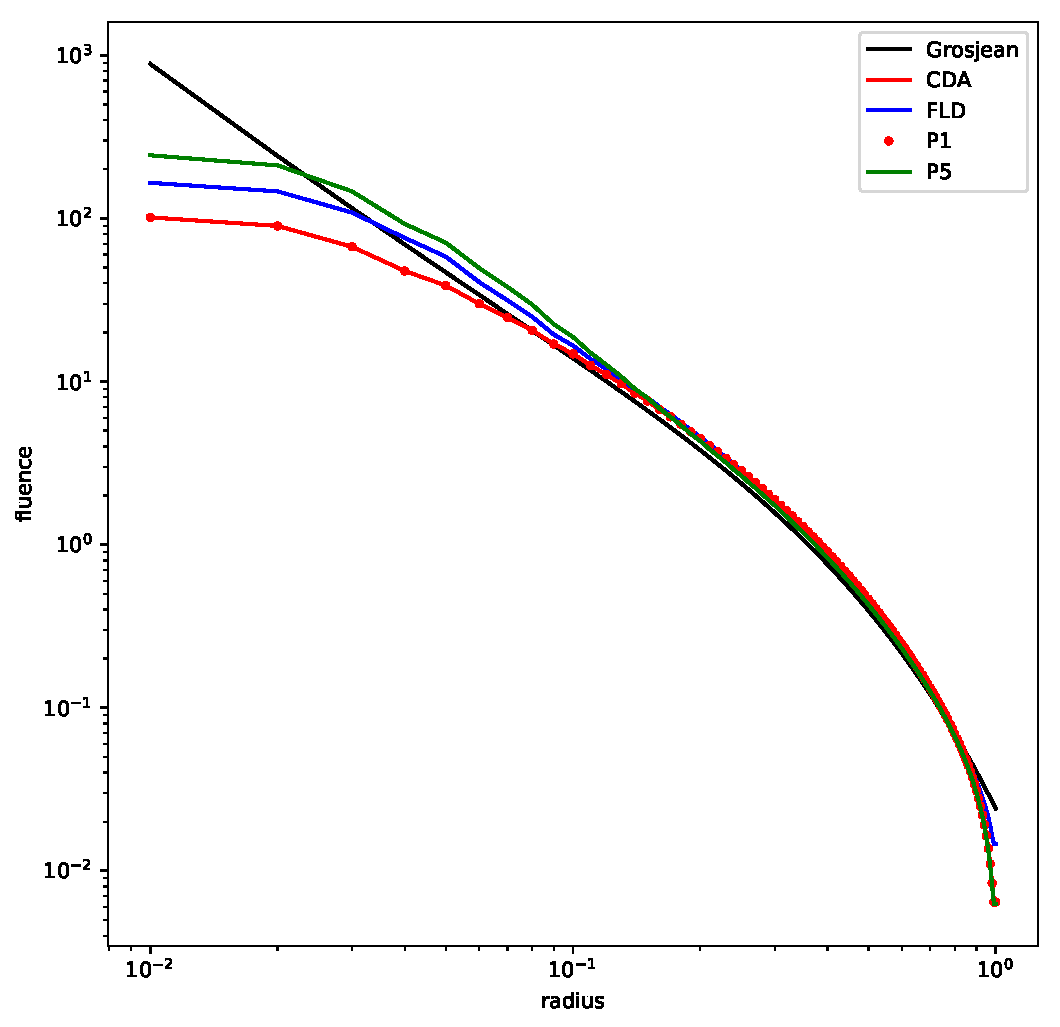
\includegraphics[width=0.7\textwidth]{06_fld/results/fld_result_plot_pointsource.pdf}
\caption{Comparing the solution from flux-limited diffusion (blue) against classical diffusion approximation (red), $P_5$-solution (green) and groundtruth (black). Flux-limited diffusion much closer to the groundtruth and $P_5$-result at much lower computational cost.}
\label{fig:fld_results_pointsource_1}
\end{figure}
As seen in figure~\ref{fig:fld_results_pointsource_1}, the result from flux-limited diffusion agree well with the ground truth and diffusion approximation results. Like with the diffusion approximation, a perfect match to the ground truth is not to be expected as flux-limited diffusion is still an approximation based on the spherical harmonics expansion of the radiative transfer equation truncated after the first moment. However, very close to the point source the flux-limited diffusion is more accurate than classical diffusion. This is explained by the fact that the fluence gradient becomes arbitrary large as the point light is approached, due to the geometry term. This causes the transport measure $R$ to likewise become arbitrary large, which shows that pure streaming transport will dominate arbitrarily close to the point source.
% figure of R: (figure~\ref{fig:fld_results_pointsource_2})

In comparison to the results from $P_N$-method and $P_5$ in particular, the $P_N$-method with higher truncation order is more accurate than flux-limited diffusion. This an important observation since it means that increasing the truncation order will alleviate the problems caused by not accounting for the flux-limit constraint. However, flux-limited diffusion has a signficicant advantage over $P_N$ due to its computational and memory efficiency.

\begin{table}[!h]
	\centering
	\caption{Performance characteristics of flux-limited diffusion for the point source problem.}
	\label{tab:results_pointsource}
	% \flushleft
	\begin{tabular}{l r}
    \hline
	\textbf{N}
    & 1
    \\
    \hline
    Number of rows/columns in $A$
    & 262.144
    \\
    Size of linear system (in MB)
    & 1.3
    \\
    Solve time (in s)
    & 34
	\end{tabular}
\end{table}

%\subsection{Checkerboard Problem}
%\label{sec:pn_results_checkerboard}
%
%For the checkerboard problem, the hand-crafted stencil for flux-limited diffusion had been modified to ignore all derivative terms in the %z-dimension. The results in figure~\ref{fig:fld_results_checkerboard_1} show how...
%\TD{discuss fld solution on checkerboard}
%\begin{figure}[h]
%\centering
%\begin{subfigure}{0.49\columnwidth}
%%\includegraphics[width=\columnwidth]{images/checkerboard2d_p1_neumann_staggered_starmap.png}
%\missingfigure{checkerboard plots FLD}
%\caption{TODO}
%\label{fig:fld_results_checkerboard_1}
%\end{subfigure}%
%\hspace{0.01\columnwidth}
%\begin{subfigure}{0.49\columnwidth}
%%\includegraphics[width=\columnwidth]{images/checkerboard2d_p1_neumann_staggered.png}
%\missingfigure{checkerboard plots CDA for comparison}
%\caption{TODO}
%\label{fig:fld_results_checkerboard_2}
%\end{subfigure}%
%\caption{TODO}
%\label{fig:fld_results_checkerboard}
%\end{figure}

\subsection{Procedural Cloud}
\label{sec:pn_results_clouds}

Finally the flux-limited diffusion is run on the procedural cloud dataset described in section~\ref{sec:pn_results_clouds} to assess how it performs in a more practical setting. As seen in figure~\ref{fig:fld_results_nebulae}, flux-limited diffusion does a significantly better job at conserving energy than classical diffusion or $P_5$. This is explained by the fact that the dataset contains very strong density gradients and close-to vacuum regions in which diffusive transport is not able to capture light transport well. While $P_5$ produces better results than classical diffusion, it is somehow surprising to see how much better flux-limited diffusion is able to capture the directly lit regions of the cloud.

Further flux-limited diffusion captures the indirectly illuminated parts at the bottom of the dataset well. Here, flux-limited diffusion also offers a signficiant improvement over classical diffusion approximation. Upon close inspection and comparison with $P_5$, it can be seen that the flux-limited diffusion solution appears very flat while the $P_5$ solution exhibits finer variations which closer resemble the path-traced resuls. This is explained by the fact that the angular domain is better resolved with $P_5$. The energy-conserving nature of flux-limited diffusion still produced a result, which more closely resembles the path-traced result than $P_5$.

\begin{figure}[h]
\centering
\begin{subfigure}[t]{0.48\columnwidth}
\includegraphics[width=\columnwidth]{06_fld/results/nebulae_ms_groundtruth.png}
\caption{Path-traced}
\label{fig:fld_results_nebulae_1}
\end{subfigure}
\hspace{0.01\columnwidth}
\begin{subfigure}[t]{0.48\columnwidth}
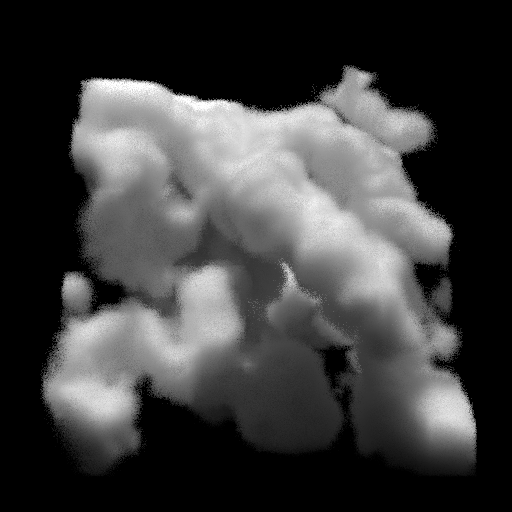
\includegraphics[width=\columnwidth]{06_fld/results/nebulae_ms_fld.png}
\caption{Flux-limited Diffusion}
\label{fig:fld_results_nebulae_2}
\end{subfigure}

\begin{subfigure}[t]{0.48\columnwidth}
\includegraphics[width=\columnwidth]{06_fld/results/nebulae_ms_cda.png}
\caption{Diffusion Approximation}
\label{fig:fld_results_nebulae_3}
\end{subfigure}%
\hspace{0.01\columnwidth}
\begin{subfigure}[t]{0.48\columnwidth}
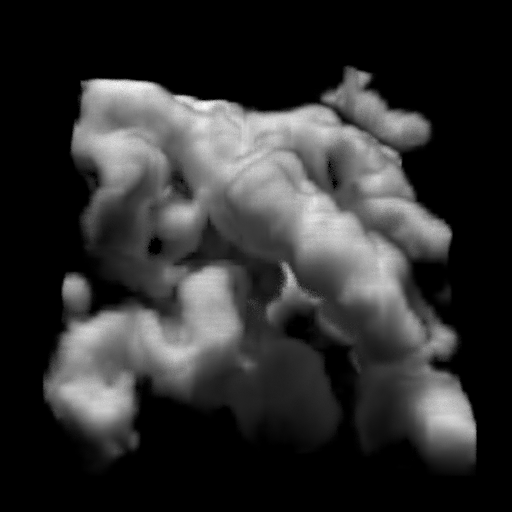
\includegraphics[width=\columnwidth]{06_fld/results/nebulae_ms_p5.png}
\caption{$P_5$}
\label{fig:fld_results_nebulae_4}
\end{subfigure}

%\vspace{-0.2in}
\caption{Flux-limited diffusion results for the procedural cloud dataset compared against previous methods. FLD produces results which are similarily close to the pathtraced solution than $P_5$ at a fraction of its computational cost.}
\label{fig:fld_results_nebulae}
\end{figure}

In terms of performance chacteristics it is to be expected that flux-limited diffusion requires more computational effort than the diffusion approximation, due to the non-linear nature of flux-limited diffusion coefficient, which must be updated for every voxel in each Gauss-Seidel iteration. This impact appears moderate when compared to the visual improvement it brings. When compared to $P_N$ it can be concluded that flux-limited diffusion offers a much better result at a significantly lower computational cost.

%\TD{complete table maybe table showing the performance characteristic for all three datasets}
%\TD{mention how the performance of FLD allows aplication of transfer function and solve for different color channels}
%\TD{mention publication}
%\TD{mention application in elementacular}
\section{Discussion}
\label{sec:fld_discussion}



\TD{write discussion}




